\documentclass{./util/unathesis}

% paquetes recomendados
\usepackage{textcomp}
\usepackage[T1]{fontenc}
\usepackage[spanish]{babel}
\decimalpoint
\usepackage[utf8]{inputenc}
\usepackage{csquotes}
\usepackage{enumerate}
\usepackage{enumitem}
\usepackage[tablename=Tabla]{caption}
\usepackage{subcaption} 
%\usepackage[style=alphabetic, uniquename=full, sorting=none, backend=biber, natbib=true, backref=true]{biblatex}
\usepackage[authoryear]{natbib}
\usepackage{listings}
% para la lista de simbolos
\usepackage{array} %for vertical thick lines in tables
\usepackage{longtable}
\usepackage{multirow} %multirow tables
\usepackage{nicefrac} %for fractions like 1/4
\usepackage[table]{xcolor} %para colorear las tablas
% para las tablas

\usepackage{listings,xcolor}

%se importan las configuraciones custmizdas realizadas.
\usepackage{tablefootnote}
\usepackage{amssymb}
\renewcommand{\thefootnote}{\arabic{footnote}}
% Macro for 'List of Symbols', 'List of Notations' etc...
\def\listofsymbols{
    \newpage
\chapter*{Lista de Símbolos\hfill}
\addcontentsline{toc}{chapter}{Lista de Símbolos}
\begin{tabbing}
% YOU NEED TO ADD THE FIRST ONE MANUALLY TO ADJUST THE TABBING AND SPACES
$n$~~~~~~~~~~\=\parbox{5in}{Vector size\dotfill \pageref{symbol:nml}}\\
%ADD THE REST OF SYMBOLS WITH THE HELP OF MACRO

%% se añaden nuevos simbolos con el macro \newsymbol y se hace referecnia
% al simbolo utilizando \addsymbol{symbol:LABEL}

\newsymbol (x_i, y_i): {coordenadas que representan un punto}{symbol:xy_i}

\end{tabbing}

    \clearpage{}
}
\def\newsymbol #1: #2#3{$#1$ \> \parbox{5in}{#2 \dotfill \pageref{#3}}\\}
\def\addsymbol#1{\label{#1}}
% Para las imagenes en grilla
% custom commands
\newcommand{\foreign}[1]{{\it #1}}
\DeclareMathOperator*{\argmax}{arg\,max}
%\algsetup{}

\usepackage{amsmath}
\usepackage{amsthm}

\newcounter{eqn}
\renewcommand*{\theeqn}{\alph{eqn}}
\newcommand{\num}{\refstepcounter{eqn}\text{\theeqn}\;}
\newcommand{\initbox}{\setcounter{eqn}{0}}

\newtheorem{definition}{Definición}

\newcommand{\figref}[1]{Figura \ref{#1}}
\newcommand{\tabref}[1]{Tabla \ref{#1}}
\newcommand{\secref}[1]{sección \ref{#1}}
\renewcommand{\algref}[1]{Algoritmo \ref{#1}}


\makeatletter
\newcommand{\putindeepbox}[2][0.7\baselineskip]{{%
    \setbox0=\hbox{#2}%
    \setbox0=\vbox{\noindent\hsize=\wd0\unhbox0}
    \@tempdima=\dp0
    \advance\@tempdima by \ht0
    \advance\@tempdima by -#1\relax
    \dp0=\@tempdima
    \ht0=#1\relax
    \box0
}}
\makeatother

%Traducción al español del paquete algorithmic%
\floatname{algorithm}{Algoritmo}
\renewcommand{\listalgorithmname}{Lista de algoritmos}
\renewcommand{\algorithmicrequire}{\textbf{Entrada:}}
\renewcommand{\algorithmicensure}{\textbf{Salida:}}
\renewcommand{\algorithmicend}{\textbf{fin}}
\renewcommand{\algorithmicif}{\textbf{si}}
\renewcommand{\algorithmicthen}{\textbf{entonces}}
\renewcommand{\algorithmicelse}{\textbf{si no}}
\renewcommand{\algorithmicelsif}{\algorithmicelse,\ \algorithmicif}
\renewcommand{\algorithmicendif}{\algorithmicend\ \algorithmicif}
\renewcommand{\algorithmicfor}{\textbf{para}}
\renewcommand{\algorithmicforall}{\textbf{para todo}}
\renewcommand{\algorithmicdo}{\textbf{hacer}}
\renewcommand{\algorithmicendfor}{\algorithmicend\ \algorithmicfor}
\renewcommand{\algorithmicwhile}{\textbf{mientras}}
\renewcommand{\algorithmicendwhile}{\algorithmicend\ \algorithmicwhile}
\renewcommand{\algorithmicloop}{\textbf{repetir}}
\renewcommand{\algorithmicendloop}{\algorithmicend\ \algorithmicloop}
\renewcommand{\algorithmicrepeat}{\textbf{repetir}}
\renewcommand{\algorithmicuntil}{\textbf{hasta que}}
\renewcommand{\algorithmicprint}{\textbf{imprimir}}
\renewcommand{\algorithmicreturn}{\textbf{retorna}}
\renewcommand{\algorithmictrue}{\textbf{cierto }}
\renewcommand{\algorithmicfalse}{\textbf{falso }}
\renewcommand{\algorithmiccomment}{\textbf{comentario : }}
\renewcommand{\algorithmicprocedure}{\textbf{Procedimiento }} 
\renewcommand{\algorithmicrequire}{\textbf{Entrada:}}

%Colores customizados
\definecolor{muybajo}{HTML}{FFF8A6}%
\definecolor{bajo}{HTML}{FAD151}%
\definecolor{normal}{HTML}{F2A82E}%
\definecolor{alto}{HTML}{A95124}%
\definecolor{muyalto}{HTML}{630C0E}%

\algsetup{indent=4em,linenosize=\small, linenodelimiter=.}

% Secciones hasta nivel 3
\setcounter{secnumdepth}{3}

% Cabeceras
\pagestyle{fancy}
\renewcommand{\chaptermark}[1]{\markboth{\MakeUppercase{\thechapter. #1 }}{}}
\renewcommand{\sectionmark}[1]{\markright{\thesection\ #1}}
\fancyhf{}
%%\fancyhead[LE,LO]{\bfseries\rightmark}
%%\fancyhead[RE,RO]{\bfseries\leftmark}
\fancyhead[LE,RO]{\chaptermark}
\fancyfoot[C]{\thepage}
\renewcommand{\headrulewidth}{0.5pt}
\renewcommand{\footrulewidth}{0pt}
\addtolength{\headheight}{0.5pt}
\fancypagestyle{plain}{
  \fancyhead{}
  \renewcommand{\headrulewidth}{0pt}
}


\makenomenclature

\makeatletter

% datos de la tesis
\degree{Informática}
\advisor{Prof. Ing.}{Joaquin Lima \\
Juan Talavera}
\logosource{./graphics/logo.png}
%\hbadness=10000
%\hfuzz=50pt
%\setcitestyle{round}

\makeatother

\begin{document}

\title{Reconocimiento de actividades humanas con un enfoque colaborativo}
\author{Alberto Gimenez \and Santiago A. Yegros Z.} 

% PDF
\hypersetup{pdftitle=Reconocimiento de actividades humanas con un enfoque colaborativo,
 pdfauthor={Alberto Gimenez, Santiago A. Yegros Z.},
 pdfsubject={Tesis de Grado}}

\maketitle     % esto hace las portadas
\frontmatter

% Agradecimientos

\chapter*{Agradecimientos}

A mis padres por estar siempre presente y brindarme la posibilidad de estudiar una carrera.

A nuestros tutores Ing. Joaquin Lima e Ing. Juan Talavera por acompañarnos y ayudarnos a llevar a cabo este trabajo.

A mi compañero de tesis, Alberto, con quien pudimos lograr sacar este trabajo de grado.

A todos los profesores que de alguna forma nos guiaron durante las materias.

A los voluntarios que nos regalaron un poco de su tiempo y esfuerzo físico para realizar las pruebas.

\begin{flushright}
	Santiago A. Yegros.Z
\end{flushright}

A mi madre Braulia por brindarme la oportunidad de tener una educación y seguir la carrera.

A mi esposa Paola y mi hija Valeria por el ánimo y las fuerzas necesarias para terminar este trabajo.

A los profesores Ing. Joaquin Lima e Ing. Juan Talavera por la guía y mentoría durante el desarrollo de este proyecto.

A los compañeros y amigos que con su entusiasmo hicieron posible culminar las pruebas.

\begin{flushright}
	Alberto Giménez
\end{flushright}


\chapter*{Resumen}

\blankpagelegend

\chapter*{Abstract}

\blankpagelegend


% los siguientes comandos producen índices.

% Tabla de contenidos
\tableofcontents	
% Lista de figuras
\listoffigures
% Lista de tablas
\listoftables
% Lista de algoritmos
\listofalgorithms

%\newpage
\chapter*{Lista de Símbolos\hfill}
\addcontentsline{toc}{chapter}{Lista de Símbolos}
\begin{tabbing}
% YOU NEED TO ADD THE FIRST ONE MANUALLY TO ADJUST THE TABBING AND SPACES
$n$~~~~~~~~~~\=\parbox{5in}{Vector size\dotfill \pageref{symbol:nml}}\\
%ADD THE REST OF SYMBOLS WITH THE HELP OF MACRO

%% se añaden nuevos simbolos con el macro \newsymbol y se hace referecnia
% al simbolo utilizando \addsymbol{symbol:LABEL}

\newsymbol (x_i, y_i): {coordenadas que representan un punto}{symbol:xy_i}

\end{tabbing}


\mainmatter  % inician los capitulos de la tesis

\nomenclature{Android}{Android es un sistema operativo móvil desarrollado por Google. Está basado en el kernel de Linux.}

\nomenclature{HAR}{Human Activity Recognition} 

\nomenclature{iOS}{Es un sistema operativo móvil creado y desarrollado por Apple Inc.}

\nomenclature{GPS}{Global Positioning System}

\nomenclature{API}{Application Programing Interfaces}

\nomenclature{SaaS}{Sofware as a Service}

\nomenclature{DT}{Decision Trees}

\nomenclature{RF}{Random Forest}

\nomenclature{SVM}{Support-Vector Machines}

\nomenclature{NB}{Naive Bayes}

\nomenclature{HMM}{Hidden Markov Models}

\nomenclature{ANN}{Artificial Neural Networks}

\nomenclature{k-NN}{k-Nearest Neighbors}

\nomenclature{HRM}{Heart Rate Monitor}

\nomenclature{Wearables}{Dispositivos o aparatos que pueden ser atuendos de un individuo}

\nomenclature{ML}{Machine Learning}

\nomenclature{Hz}{Hertz, unidad de medida de ciclos por segundo}

\nomenclature{WIFI}{Wireless Fidelity, permite tener acceso o conectarse a una red utilizando ondas de radio}

\nomenclature{Bluetooth}{Estándar para red personal}

\nomenclature{GPRS}{General Packet Radio Service, servicio de datos moviles en comunicaciones celulares 2G/3G}

\nomenclature{GSM}{Global System for Mobile, sistema de comunicación celular global.}

\nomenclature{3G}{Tercera generación de sistema de comunicación celular.}

\nomenclature{4G}{Cuarta generación de sistema de comunicación celular.}

\nomenclature{SMS}{Short Message Service}

\nomenclature{MMS}{Multimedia Messaging Service}

\nomenclature{Kinect}{Sensor de profundidad de Microsoft}

\nomenclature{WGS}{World Geodetic System}

\nomenclature{FFT}{Fast Fourier Transform}

\nomenclature{FV}{Feature Vectors}

\nomenclature{Smartphones}{Teléfonos inteligentes}

\nomenclature{Smartwatches}{Relojes Inteligentes}

\nomenclature{IPC}{Inter Process Communication}

\nomenclature{CPU}{Central Processing Unit}

\nomenclature{GPU}{Graphical Processing Unit.\\}

\nomenclature{Kernel}{Núcleo principal de un sistema operativo moderno.}

\nomenclature{Linux}{Proyecto de software libre para producir un núcleo de sistema operativo basado en Unix}

\nomenclature{HAL}{Hardware Abstraction Layer}

\nomenclature{DVM}{Dalvik Virtual Machine}

\nomenclature{JVM}{Java Virtual Machine}

\nomenclature{Java}{Lenguaje de programación orientado a objetos}

\nomenclature{SQL}{Structured Query Language}

\nomenclature{CRUD}{Create, Read, Update, Delete}

\nomenclature{URI}{Universal Resource Identifier}

\nomenclature{REST}{Representational State Transfer}

\nomenclature{UML}{Unified Modeling Language}

\nomenclature{AIDL}{Android Interface Definition Language}

\nomenclature{JAR}{Java ARchive}

\nomenclature{WEKA}{Waikato Environment for Knowledge Analysis}

\nomenclature{TP}{True Positive}

\nomenclature{TN}{True Negative}

\nomenclature{FP}{False Positive}

\nomenclature{FN}{False Negative}

\nomenclature{APK}{Android Application Package}

\nomenclature{PC}{Personal Computer}

\nomenclature{OS}{Operating System}

\nomenclature{HARDroid}{Servicio de Reconocimiento de Actividades para Android}

\nomenclature{SDK}{Software Development Kit}


% incluye aqui los capitulos (un archivo .tex por capitulo)

\chapter{Introducción}

\label{chap1:introduccion}

Hace apenas una década, que los teléfonos móviles pasaron de ser simples
aparatos de comunicación, a ser dispositivos de información que se
han extendido en todo el mundo como el dispositivo electrónico más
utilizado de manera diaria. Desde la aparición de los teléfonos móviles
modernos (\emph{Smartphones}, o teléfonos inteligentes) con pantalla
táctil, la convergencia en el uso de teléfonos móviles, las redes
de datos e Internet ha ido aumentando gradualmente \cite{Fling2009}.

La capacidad y prestaciones de los teléfonos móviles modernos han
mejorado drásticamente, ya que fusiona los aspectos de teléfonos móviles
y computadoras portátiles, la promesa esperada desde hace más de una
década \cite{Tanenbaum2010}. Muchas de las tareas asociadas comúnmente
a una computadora personal de escritorio pueden ser realizadas con
un teléfono móvil moderno, pero con la ventaja adicional de que el
móvil está más próximo a las actividades diarias del portador.

Desde los teléfonos móviles modernos se tiene acceso a la información
pero en un contexto móvil. El contexto puede darse de dos formas,
la primera forma es el valor que los usuarios mismos generan a partir
de las circunstancias en la que están involucrados. La información
provee un contexto que permite al usuario entender mejor el momento
que está experimentando. Por otro lado, el contexto también es determinado
por la acción que el usuario realizar en su entorno \cite{Fling2009}.
En este último caso, el contexto físico de un usuario involucra a
su ubicación y su actividad humana. 

El reconocimiento de actividades humanas (\abbr{HAR}, \emph{Human
Activity Recognition}) es un tópico de investigación que busca diseñar
algoritmos que provean información acerca del contexto de uno o más
individuos a partir de datos ambiguos capturados en su entorno \cite{Bao2004}.
Reconocer el contexto es un componente primordial de los sistemas
inteligentes y cognitivos, este forma parte de un proceso más complejo,
donde contribuye en las etapas de análisis y captura de datos a través
de sensores externos o adjuntos a los individuos \cite{ReyesOrtiz2015,Chen2012}.
Los avances recientes en las tecnologías de computación móvil y sensores
tales como: la miniaturización, bajo consumo, buenas prestaciones,
buena conectividad y el procesamiento de datos, hizo que proliferara
el uso de los teléfonos móviles modernos con sistemas inteligentes
que monitorizan las acciones del usuario en su vida diaria. 

Diseñar sistemas móviles inteligentes, o aplicaciones móviles de contexto,
que reconozcan las actividades de un individuo, Ej. Si está caminando,
está corriendo, está quieto o moviéndose en algún vehículo tiene diversos
motivos en la actualidad \cite{CampuzanoLopez2015,Google2013l}. Tal
es la motivación, que ha aumentado la popularidad de las aplicaciones
móviles de contexto con funcionalidades en el ámbito del cuidado personal,
la movilidad y la asistencia en la vida diaria que requieren de estas
capacidades. Por citar ejemplos, en la actualidad existen diversas
alternativas en el mercado, como las proveídas por las grandes compañías
\emph{Google}, \emph{Sony} y \emph{Apple}, que son principales fabricantes
de teléfonos móviles e impulsores aplicaciones móviles basadas en
contexto.

Desde el año 2013, \emph{Google} ha proveído como complemento para
la plataforma \emph{\abbr{Android} }\cite{Google2005a} el producto
\emph{Google Play Services}, este dispone de una librería para el
reconocimiento de actividades humanas exclusivamente para desarrolladores
de aplicaciones móviles \cite{Google2013l}. Saliendo al paso, \emph{Sony}
ha lanzado una suite completa (aplicaciones móviles, pulseras y relojes)
para mantenerse en forma acompañados del producto \emph{Lifelog} \cite{Sony2016l}.
Este también es capaz de reconocedor de actividades físicas y registrar
las acciones de sus usuarios simplemente portando el teléfono en cualquier
lugar. Además, \emph{Apple} para su plataforma\emph{ \abbr{iOS}}
\cite{Apple2007i} ha dispuesto recientemente de una librería para
desarrolladores llamada \emph{HealthKit} \cite{Apple2016h}, con un
enfoque similar a los productos anteriormente mencionados. 

Las plataformas para aplicaciones \emph{\abbr{Android}} e \emph{\abbr{iOS}}
proveen un ecosistema abierto para crear aplicaciones personalizadas,
estas conducen a la expansión y el crecimiento de aplicaciones contextuales
\cite{Tanenbaum2010}. Sin embargo, a pesar de promoverse plataformas
abiertas, existe aún una carencia de proyectos colaborativos de código
abierto que contribuyan al desarrollo de sistemas inteligentes de
contexto, a excepción de ciertos precedentes (véase \cite{Kwapisz2011,LaraLabrador2013})
que han hecho esfuerzos iniciales u otras iniciativas como \cite{FUNF2016}
y \cite{SensingKit2016} orientados a la colaboración.

Desde que los teléfonos móviles modernos conectados constantemente
Internet el acceso a la Web\footnote{World Wide Web} se ha popularizando.
Esto impulsó a que la computación móvil haya crecido enormemente,
y también ha crecido el uso de la Web (cfr. \cite{NYTimes2008iph}).
Esto fomenta un ámbito de trabajo colaborativo, distribuido y móvil
donde un grupo masivo de personas pueden aportar a un propósito común,
ya sea como sujetos de estudio en el reconocimiento de actividades
humanas o en el desarrollo de herramientas para aplicaciones móviles
contextuales.

\section{Planteamiento del problema}

\label{sec11:planteamiento}

El reconocimiento de actividades humanas es un tópico de investigación
que data desde los noventa (90), y a la actualidad sigue atrayendo
bastante interés ya que abarca varias áreas novedosas de estudio.
Algunas áreas de estudio que se pueden mencionar son la computación
ubicua, la computación móvil, y la computación contextual; también
la seguridad por vigilancia, las viviendas asistidas y los ambientes
inteligentes, etc.\cite{Chen2012}. 

Reconocer actividades humanas consiste en detectar las acciones o
interacciones con el entorno que llevan acabo las personas utilizando
sensores. Las actividades humanas pueden ser catalogados en distintos
tipos y según el nivel de detalle \cite{Chen2012}. Poniendo énfasis
en las actividades básicas que un individuo puede realizar podemos
destacar las acciones físicas más simples, como lo son las actividades
ambulatorias y de transportación. Además existen otras acciones más
complejas como la postura, los movimientos en ejercicio aeróbico u
otras más seculares, Ej. Cepillarse los dientes, mirar televisión,
comer, beber, hablar por teléfono, etc. \cite{LaraLabrador2013}.

El problema del reconocimiento de actividades humanas conlleva un
proceso complejo que se resume en la utilización de técnicas de aprendizaje
automático supervisado, con un modelo de inferencia construido en
dos etapas: entrenamiento y evaluación \cite{LaraLabrador2013,Kwapisz2011}.
Es un proceso se puede resumir en un flujo iterativo que consiste
en \cite{Bao2004}:
\begin{itemize}
\item Recolectar datos etiquetados de un conjunto de individuos de forma
supervisada. 
\item Extraer variables predictoras con atributos relevantes al estudio.
\item Construir un modelo de predicción de actividades humanas.
\item Detectar con cierta precisión el conjunto de actividades previamente
etiquetadas utilizando como entrada un conjunto de datos no etiquetados.
\item Retroalimentar y/o evaluar el modelo para obtener una mejora continua.
\end{itemize}
La investigación en el área de los sistemas \abbr{HAR} utilizando
teléfonos móviles ha progresado de manera sostenida debido a los avances
tecnológicas de sensores de bajo costo, las redes inalámbricas de
alta velocidad y los dispositivos móviles inteligentes \cite{Chen2012}.
A pesar de los avances tecnológicos, aún existen importantes desafíos
por resolver como: seleccionar medidas relevantes, recolectar datos
en forma no invasiva, analizar métodos de inferencia alternativos
y extraer muestras significativas \cite{LaraLabrador2013}. Además
de la restricción al recolectar datos en condiciones realistas y tener
la flexibilidad para soportar nuevos individuos sin necesidad entrenar
el modelo permanentemente se debe diseñar el sistema bajo condiciones
especiales de ahorro de energía y procesamiento \cite{ReyesOrtiz2015}. 

De las cuestiones citadas anteriormente, en este trabajo ponemos énfasis
en cuatro puntos que enmarcan el problema a resolver y cuya justificación
responde a utilizar los teléfonos móviles como plataforma de reconocimiento
de actividades humanas.

\section{Justificación}

\label{sec12:justificaciuxf3n}

Para construir sistemas \abbr{HAR} se requiere utilizar uno o más
sensores que midan datos del entorno de un usuario. Los teléfonos
móviles modernos poseen múltiples sensores de bajo consumo, con el
tamaño y las condiciones adecuadas para la capturar de manera ubicua.
Comúnmente los teléfonos modernos se componen de sensores de: localización
(\abbr{GPS}, \emph{Global Positioning System}), brújula, aceleración,
audio (micrófonos) y vídeo (cámaras), luminosidad, temperatura, barómetro
y otros dependiendo del fabricante y/o accesorios adicionales\cite{Kwapisz2011}.

El sensor de aceleración\footnote{acelerómetro} mide el movimiento
en dos o tres ejes y puede ser combinado con otros para detectar la
orientación del dispositivo. Estas medidas proveen información crucial
para el reconocimiento de actividades humanas con un bajo consumo
de energía. El sensor de localización y podómetro (contador de pasos)
también son ideales para su uso pero poseen más restricciones asociadas.
Adicionalmente, los teléfonos modernos tienen capacidad de almacenamiento
y procesamiento, una buena conectividad por lo que son plataformas
ideales para construir sistemas de reconocimiento autónomos.

La combinación de capacidad, tamaño diminuto y bajo costo hace que
los dispositivos sean portados a cualquier lugar por sus usuarios,
esto permite recolectar los datos en condiciones realistas, una ventaja
ideal que tener que obtener muestras supervisadas en un laboratorio
\cite{Bao2004}. 

La información sobre el estado de arte de esta área de investigación
es bastante extensa y abarca las técnicas de reconocimiento, los métodos
de captura y el procesamiento de datos de sensoriales\cite{LaraLabrador2012,Kwapisz2011}.
Sin embargo, a pesar de estar definida la arquitectura los sistemas
\abbr{HAR}, aún existe un hueco de contar con un componente de software
para teléfonos móviles que pueda ser utilizado sin depender de librerías
privadas, Ej. \emph{Google Play Services} API \cite{Google2016l}
(\abbr{API}, \emph{Application Programming Interface}), o servicios
alojados en Internet (\abbr{SaaS}, \emph{Software as a Service}),
o bien aplicaciones distribuidas por terceros, Ej. \emph{Lifelog}.

El modelo de desarrollo de software libre hace posible tener un enfoque
colaborativo en dos dimensiones, por un lado el software como tal,
Ej. Una librería de reconocimiento, y por otro el los de datos sensoriales
utilizadas para el entrenamiento del modelo de predicción de actividades.

\section{Alcance y Objetivos}

\label{sec13:alcance-y-objetivos}

Este trabajo se centra en el reconocimiento de actividades humanas
con teléfonos móviles inteligentes utilizando sensores y aportar una
componente de librería de código abierto que sea libremente distribuida.
Durante la recolección de datos y las pruebas se desarrollará adicionalmente
una aplicación móvil que demuestre la efectividad de la librería como
componente de software independiente. También se evaluará el sistema
de reconocimiento de actividades basado en aprendizaje automático.

Se incluye la revisión del estado del arte de la materia con el objetivo
de comprender las metodologías de reconocimiento actualmente empleadas.
Luego, se construirá una librería cliente y un servicio basado en
\emph{\abbr{Android}} que atienda a las llamadas de procedimiento
del sistema de reconocimiento de actividades. 

Dentro del sistema de reconocimiento se incluirá un modelo colaborativo
capaz de actualizarse constantemente, a nuestro criterio, esto mejorará
las predicciones basándose en un conjunto de datos de entrenamiento
proveniente de las personas que colaboren de forma anónima y en condiciones
reales.

Además se implementará un servicio Web de captura de muestras con
predicciones para evaluar y actualizar el modelo de predicción para
futuras versiones. El modelo de aprendizaje se basará en aprendizaje
automático por árboles de decisión (\abbr{DT}, \emph{Decision Trees}).
Finalmente, para evaluar la metodología se creará una aplicación móvil
para recolectar muestras y evaluar el resultado de predicción utilizando
el sistema de reconocimiento propuesto.

\subsection{Objetivo General}

\label{sec13:objetivo-general}

Implementar un sistema de reconocimiento de actividades humanas con
teléfonos móviles cuyo principal aporte sea una librería de código
abierto libremente distribuido.

\subsection{Objetivos Específicos}

\label{sec13:objetivos-especuxedficos}
\begin{enumerate}
\item \label{enu:obe1}Definir el estado del arte sobre reconocimiento de
actividades humanas (\abbr{HAR}). 
\item \label{enu:obe2}Comprender las técnicas de recolección de datos en
entornos restringidos para bajo consumo energía. 
\item \label{enu:obe3}Comprender el procesamiento de señales de datos de
aceleración inercial para identificar variables significativas de
entrenamiento. 
\item \label{enu:obe4}Comprender la clasificación por aprendizaje automático
en entornos restringidos para bajo consumo energía. 
\item \label{enu:obe5}Diseñar un sistema de reconocimiento de actividades
que comprenda la recolección de muestras de manera colaborativa y
predicción de actividades en-línea. 
\item \label{enu:obe6}Aportar un componente de software de código abierto
para uso en teléfonos móviles inteligentes. 
\end{enumerate}

\section{Organización del trabajo}

\label{sec14:organizaciuxf3n-del-trabajo}

El trabajo está organizado en la siguiente manera: en el Capítulo
2 se presenta define el marco teórico del área describiendo los conceptos
principales del reconocimiento de actividades humanas, sus características,
dificultades, y las metodologías existentes. El Capítulo 3 definimos
el aprendizaje automático, los tipos de aprendizajes, y las distintas
técnicas o enfoques aplicados, dando énfasis en los arboles de decisión.
Estos capítulos representan el estado del arte de este trabajo.

El Capítulo 4 se presenta en detalle la construcción de un sistema
de reconocimiento para teléfonos móviles. Continuando, en el Capítulo
5 se discute el modelo y la implementación de un reconocedor de actividades
colaborativo, su diseño, arquitectura, y tecnologías utilizadas.

En el Capítulo 6 se detallan los protocolos de los experimentos realizados,
y en el Capítulo 7 los resultados obtenidos durante el estudio. Para
finalizar, en el Capítulo 8 se incluyen las conclusiones y los posibles
trabajos futuros. 
 	%Cap 1: Introducción
%Parte II: Marco referencia (Background): 

\chapter{Marco Teórico}

\label{chap2:marco-teorico}

\section{Introducción}

\label{sec21:introduccion}En este capitulo, se resumen las cuatro
áreas principales de estudio relacionados a los sistemas \abbr{HAR}
con miras a definir el problema del reconocimiento de actividades
humanas desde un punto de vista teórico. La descripción de estas áreas
detallan las aplicaciones que motivan los sistemas \abbr{HAR} y también
los mecanismos que llevan a una implementación factible. 

La primera sección, se introducen las aplicaciones de contexto que
son el principal marco de trabajo del estudio de sistemas \abbr{HAR}.
En síntesis, nuestro enfoque es detectar las actividades físicas para
dar información de contexto en las actividades diarias de un individuo
durante su locomoción. Las siguientes secciones dan todos los elementos
requeridos para implementar los sistemas \abbr{HAR}. Desde el punto
de vista de implementación se discuten los sensores y los teléfonos
móviles inteligentes. La última sección define el marco teórico del
reconocimiento de actividades humanas en base al estado de arte.

\section{Aplicaciones de contexto}

\label{sec22:contexto}En la actualidad construir aplicaciones interactivas
requieren tener en cuenta el aspecto del contexto del usuario principalmente
por la importancia de este asunto debido a que este cambia con mucha
frecuencia, como ocurren en la computación móvil y ubicua. El contexto
de un usuario es un medio adicional para la interacción entre computadora
y humano, además de otros los métodos convencionales de entrada de
datos. Este nuevo medio abre nuevas posibilidades de comunicación
y producción de nuevos servicios en computación. 

Pero, ¿qué es el contexto?, citando otras fuentes podemos definir
el contexto como: \textquotedbl{}\emph{... cualquier información que
pueda ser utilizada para caracterizar la situación de una entidad.
Un entidad es una persona, lugar, o objeto que es considerado relevante
en la interacción entre el usuario y la aplicación, incluyendo al
usuario y la aplicación}\textquotedbl{} \cite{Dey2000}. De manera
específica, el contexto de un usuario es el estado de su información
física, emocional o social, sin dejar de lado cualquier otra situación
en que el usuario esté involucrado y sea relevante para la aplicación.

Debido a la libertad de movilidad presentes en la computación móvil
y ubicua, es primordial construir aplicaciones que conozcan el contexto
de sus usuarios (\emph{context-aware}, o aplicaciones de contexto).
Debido a que el entorno de ejecución cambia con cierto dinamismo,
el rango de situaciones posibles del usuario se amplia y por lo tanto
se requiere que los servicios proveídos por una aplicación se adapten
para mejorar la interacción entre el usuario y el computador. 

Los tipos de contexto prácticos más importantes en las aplicaciones
de contexto con computación móvil son la ubicación, la identidad,
la actividad y el tiempo. Esta caracterización permite a los diseñadores
de aplicaciones escoger el contexto más relevante para su uso.

\section{Sensores}

\label{sec23:sensores} En la problemática del reconocimiento de actividades
realizada por un individuo, uno de los temas importantes a tratar
es la elección de los sensores utilizados. Se han utilizando sensores
variados para extraer información acerca de las actividades de un
individuo. Los sensores pueden medir signos vitales (ritmo cardíaco,
temperatura del cuerpo, presión arterial), señales del ambiente (intensidad
de luz, temperatura, niveles de sonido), el movimiento (aceleración,
velocidad), y la posición (localización global o en interiores). 

Con respecto a la disposición de los sensores en relación a los usuarios,
algunos autores \cite{ReyesOrtiz2015,LaraLabrador2013} diferencian
entre ambientales, los sensores están ubicados de fija en el ambiente
que rodea a al individuo, y \emph{wearables} cuando los sensores están
puestos o conectados al cuerpo de la persona.

\subsection{Sensores Ambientales}

Los sensores ambientales, también denominados externos o de entorno,
son un conjunto de dispositivos que se encuentran en el entorno y
miden propiedades físicas del mismo, a las personas que rodean, y
la interacción entre los mismos. Existe una amplia variedad de sensores
ambientales, como micrófonos, cámaras de vídeo, sensores de presencia,
termómetros y sensores de profundidad (Ej. \abbr{Kinect}). 

Existen varios trabajos que explorar el uso de sensores ambientales
para reconocimiento de actividades. Entre ellos el lo expuesto por
\cite{Poppe2007} que realiza un análisis de movimientos humanos utilizando
cámaras de vídeo. A pesar de ser bastantes efectivos los sistemas
basados en vídeos existen grandes limitaciones para procesamiento
en tiempo real y la privacidad de los usuarios.

\subsection{Sensores Wearables}

Los sensores \emph{wearables} (o de atuendo) son utilizados para obtener
señales directamente de los usuarios, los sensores pueden estar anexos
a varias partes del cuerpo, como la cintura, la muñeca, el pecho,
la pierna, y la cabeza \cite{Bao2004} como también pueden formar
parte de alguna vestimenta. También, pueden estar embebidos en algún
accesorio de uso común, como relojes, anteojos y los teléfonos móviles. 

Como característica adicional tienen autonomía gracias al uso de baterías
que proporcionan energía para poder operar, y además algunos cuentan
con conexiones inalámbricas (Ej. \abbr{WIFI}/\abbr{Bluetooth}) para
la transmisión de las señales. Las señales de movimiento y fisiológicas
obtenidas por los sensores pueden ser temperatura de la piel, frecuencia
cardíaca, conductividad, posicionamiento global (\abbr{GPS}) y movimientos
del cuerpo. Todos estas mediciones son útiles para tener una constante
información del estado de una persona en cualquier momento.

Los sensores anexos directamente a un individuo se clasifican comúnmente
según los siguientes grupos \cite{LaraLabrador2013}:
\begin{description}
\item [{Movimiento}] miden datos inerciales como la aceleración y la orientación
respecto a un marco de referencia relativo al dispositivo que contiene
los sensores. El acelerómetro, giroscopio y la brújula son los sensores
más comunes y utilizados para reconocimiento de actividades con un
bajo consumo de energía y buena precisión de reconocimiento \cite{Bao2004,LaraLabrador2012}.
\item [{Ubicación}] miden datos obtenidos con las redes celulares 3G y
los satélites de navegación \abbr{GPS}. Provee información de contexto
bastante relevante acerca de la posición del individuo, además de
ciertas medidas de movimiento pero con un consumo moderado de energía.
\item [{Fisiología}] miden signos vitales del individuo como el ritmo cardíaco
(\abbr{HRM}, \emph{Hearth Rate Monitor}), la temperatura del cuerpo,
el ritmo de respiración, entre otros.
\item [{Ambiente}] miden datos externos que rodean al individuo como el
nivel de ruido, la humedad y/o la temperatura. Los sensores de luz,
cámara, micrófonos y termómetros miden estas señales. 
\end{description}

\section{Dispositivos móviles}

\label{sec24:dispositivos-moviles} Los dispositivos móviles, tales
como teléfonos móviles, reproductores de música o relojes inteligentes,
han comenzado ya hace un par de años en incorporar diversos sensores.
Debido a su tamaño reducido de estos dispositivos inteligentes, su
enorme capacidad de procesamiento, la posibilidad de recibir y enviar
datos; y su omnipresencia en nuestra sociedad de hoy, lo hacen dispositivos
de preferencia para utilizarlo en la vida diaria de un usuario.

En este trabajo, investigamos posibilidades y viabilidades de tener
un servicio para obtener el contexto de la actividad física diaria
de los usuarios con teléfonos móviles.

%% TODO: Definir mejor los teléfonos móviles, no tanto los sensores

\section{Aprendizaje Automático}

\label{sec25:aprendizaje-automatico}Una de las técnicas de reconocimiento
de actividades humanas consiste en encontrar un modelo para descubrir
información a partir de los datos, es decir utilizar algoritmos de
aprendizaje automático (\abbr{ML}, \emph{Machine Learning}) para
construir modelos que puedan inferir actividades a partir de una gran
cantidad de datos medidos con anterioridad junto con el comportamiento
deseado del usuario\cite{Chen2012}. Esta técnica involucra la creación
de modelos de clasificación probabilistas o estadísticos, seguidos
por los procesos de entrenamiento y aprendizaje.

El aprendizaje automático implica la utilización de datos como conjunto
inicial de entrenamiento para entrenar un algoritmo, uno de muchos
existentes, como redes de Bayes, máquinas de soporte-vector \abbr{SVM},
Árboles de decisión \abbr{DT}, Modelos de Markov ocultos\abbr{HMM},
y otros \cite{Rajaraman2011} (véase siguiente sección). Las ventajas
de utilizar este enfoque de reconocimiento es su capacidad de manejar
información temporal y con cierto grado de incertidumbre, pero su
desventaja es que requiere una cantidad grande de datos de entrenamiento,
por lo que puede sufrir de problemas de inicio lento y escasez de
datos.

\section{Reconocimiento de Actividades Humanas}

El campo de estudio del \abbr{HAR} incluye las metodologías para
comprender el comportamiento humano a partir de interpretar atributos
derivados de diversas fuentes \cite{Bao2004,Poppe2007}, como por
ejemplo el movimiento con sensores, ubicación u otras señales fisiológicas. 

El objetivo es identificar las acciones llevadas acabo por una persona
en base a observaciones realizadas sobre el mismo en el entorno que
se desenvuelve. Las aplicaciones en computación móvil y ubicua explotan
el contexto del usuario haciendo uso de sistemas \abbr{HAR} como
una herramienta tecnológica. Para tener un conocimiento acabado de
este trabajo, en esta sección se expone una descripción general de
aspectos clave como la definición del problema, el proceso de reconocimiento
estándar, las actividades estudiadas y las técnicas de aprendizaje.

\subsection{Definición del Problema}

\label{sec261:definicion-har}De manera a establecer el marco teórico
de estudio del problema \abbr{HAR} en este apartado se describe una
definición formal del problema. Considerando el objetivo y los elementos
de reconocimiento podemos definir el problema como\cite{LaraLabrador2013}:

\newtheorem{defi}{Definición}

\begin{defi}(Problema \abbr{HAR}) Dado un conjunto $S=\{S_{0},...,S_{k-1}\}$
de $k$ series de tiempo, cada una con una medida particular de cada
atributo, y definidas en el intervalo de tiempo $I=\left[t_{\alpha},t_{\omega}\right]$,
el objetivo es encontrar una partición temporal (sub-intervalo de
tiempo) $\left\langle I_{0},...,I_{r-1}\right\rangle $ en $I$, basado
en los datos de $S$ y el conjunto de etiquetas que representan la
acción realizada durante cada intervalo $I_{j}$ (Ej. quieto, caminando,
corriendo, etc.). 

Esto implica que cada intervalo $I_{j}$ son consecutivos, no vacíos,
no superpuestos y que ${\displaystyle \bigcup_{r-1}^{j=0}{I_{j}=I}}$
\end{defi}

Se asumen que las acciones consideradas no son realizadas simultáneamente,
es decir la persona no realiza la acción de correr y caminar al mismo
tiempo. Además, se debe notar que el problema \abbr{HAR} no es factible
a ser resuelto con una solución determinista. El numero de combinaciones
de valores de atributos y acciones puede ser muy grande, inclusive
infinito; y encontrar los puntos de transición es complejo teniendo
en cuenta que se desconoce la duración cada acción. 

Es por esta razón que las metodologías de aprendizaje automático son
utilizadas como proceso para reconocer actividades humanas por medio
de la técnica clasificación. Debido a la utilización de aprendizaje
automático para la resolución del problema, se requiere la siguiente
definición relajada del problema \abbr{HAR} descrito anteriormente: 

\newtheorem{defi}{Definición}

\begin{defi}(Problema \abbr{HAR} relajado) Dado (1) un conjunto
$W=\{W_{0},...,W_{m-1}\}$ de $m$ ventanas de tiempo del mismo tamaño,
donde cada una está total o parcialmente etiquetada, y que cada $W_{i}$
contiene un conjunto de series de tiempo $S_{i}=\{S_{i,0},...,S_{i,k-1}\}$
para cada $k$ atributos medidos, y (2) un conjunto $A\text{=}\{a_{0},...,a_{n-1}\}$
de etiquetas de actividades, el objetivo es encontrar una función
$f\colon S_{i}\rightarrow A$ que sea evaluada para todos los valores
posibles de $S_{i}$, tal que $f(S_{i})$ es lo más próximo a la acción
realizada durante $W_{i}$ \end{defi}

Considerar la utilización de esta definición relajada introduce un
error en el modelo durante las ventanas de transición entre actividades,
debido a que, en una ventana de tiempo una persona puede estar realizando
más de una acción. Sin embargo, el número de ventanas en transición
es menor al número total de ventanas por lo que el error introducido
por relajar el problema no es significativo para la mayoría de las
aplicaciones.

\subsection{Proceso de Reconocimiento }

\label{sec262:proceso-har}Al igual que en otras aplicaciones de aprendizaje
automático, el proceso de reconocimiento se divide en dos etapas bien
conocidas, la de entrenamiento y las pruebas (o evaluación).

\begin{figure}[!htbp]
\centering 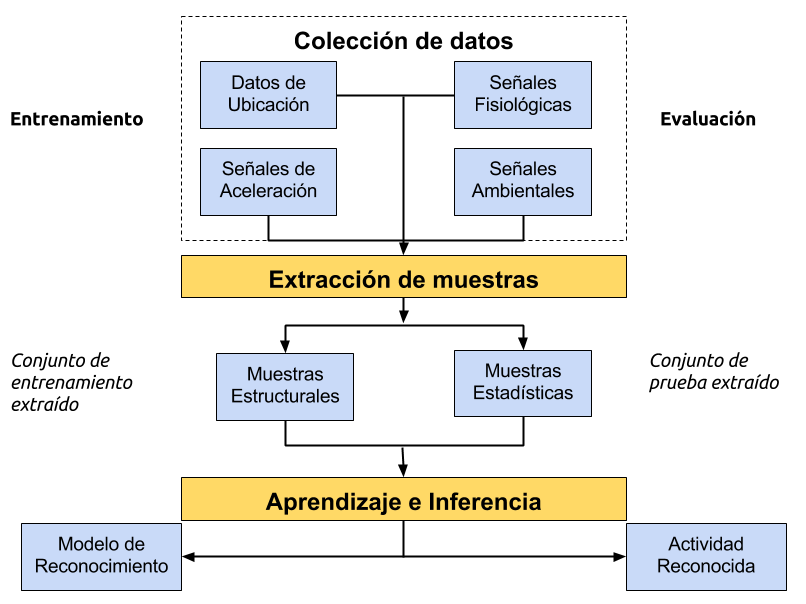
\includegraphics[width=0.7\linewidth]{capitulo-2/graphics/harsystem}
\caption[Flujo HAR]{Flujo general del Reconocimiento de Actividades Humanas}
\label{fig:harsystem} 
\end{figure}

En la \figref{fig:harsystem} se visualiza las fases comunes de las
dos etapas \cite{LaraLabrador2013}. La etapa de entrenamiento requiere
inicialmente un conjunto de datos recolectados en una serie de tiempo
con los atributos medidos a partir de individuos que realizan cada
actividad. Las series se dividen en ventanas de tiempo para aplicar
la extracción de muestras filtrando así la información relevante en
las señales en bruto. 

Más adelante, se utilizan métodos de aprendizaje para generar un modelo
de reconocimiento de actividades a partir del conjunto de datos colectado
a través de las características calculadas. Del mismo modo, para la
etapa de prueba o evaluación, se recogen datos durante una ventana
de tiempo, que se utiliza para extraer las mismas características
utilizadas en el modelo, estas se evalúan en el modelo de aprendizaje
previamente entrenado, generando una etiqueta de la actividad predicha.

En las siguientes secciones detallamos el objeto de la clasificación
(actividades humanas) y las funciones de cada etapa.

\subsection{Actividades Humanas}

\label{sec263:actividades-humanas} El diseño e implementación de
un sistema \abbr{HAR} depende totalmente de las actividades que serán
reconocidas. Por lo tanto, el cambio del conjunto de actividades que
un sistema reconoce convierte al problema en uno completamente distinto
a otro sistema construido con el mismo propósito.

Teniendo en cuenta esta razón, y de acuerdo a distintas publicaciones,
presentamos siete grupos distintos de actividades agrupados en la
siguiente tabla.

\begin{table}[htbp]
\centering{}%
\begin{tabular}{|l|p{9cm}|}
\hline 
\textbf{Grupo}  & \textbf{Actividades} \tabularnewline
\hline 
\hline 
Ambulatoria  & Caminar, correr, sentarse, pararse, quedarse quieto, acostarse, subir
escaleras, descender escaleras, usar escaleras mecánicas, usar elevador.\tabularnewline
\hline 
Transporte  & Andar en bus, bicicleta y conducir \tabularnewline
\hline 
En el teléfono  & Enviar mensajes de texto y hacer llamadas \tabularnewline
\hline 
Actividades diarias  & Comer, beber, trabajar en la PC, mirar TV, leer, cepillarse los dientes,
aspirar el piso, y otros. \tabularnewline
\hline 
Ejercitarse  & Alzar pesas, bicicleta estática, remo y otros. \tabularnewline
\hline 
Militares  & Arrastrarse, en cuclillas, abrir la puerta \tabularnewline
\hline 
Parte superior del cuerpo  & Masticar, hablar, mover la cabeza, tragar líquidos, mirar. \tabularnewline
\hline 
\end{tabular}\caption{Grupos de Actividades.}
\label{tabla:sencilla} 
\end{table}

Las actividades pueden separase en varios grupos de acuerdo a la duración
y la complejidad del evento. Los eventos cortos son movimientos de
transición y movimientos en base a gestos. Los eventos al que nos
enfocamos en este trabajo son aquellos que se componen de las actividades
básicas de larga duración que se caracterizan por las acciones continuas
y cíclicas de un individuo \cite{ReyesOrtiz2015}. Nuestro estudio
no se basa en actividades complejas que sean una secuencia de actividades
básicas y eventos cortos.

Definimos como objetivo de estudio detectar actividades básicas ambulatorias
y de transporte, de larga duración y sin cambios bruscos de transición.

\subsection{Colección de Datos}

La definición del método de colección de datos es un punto importante
en un sistema \abbr{HAR}. Según como se realiza la observación del
individuo existen: ambientes realistas, que son los ideales pero no
siempre es posible realizar este tipo de colectas. También existen
los ambientes cuasi realistas que se realizan en laboratorios simulando
las condiciones reales de las actividades. Por otro lado tenemos los
ambientes totalmente controlados en laboratorio.

Una falla en el diseño de un sistema \abbr{HAR} se puede dar por
no considerar las condiciones reales de las actividades, tales como
actividades no tenidas en cuenta, calibración de sensores, ruido,
etc.

Otra de las consideraciones a tener en cuenta en este punto es la
cantidad de individuos para realizar la colección, es recomendable
el mayor cantidad de individuos en distintos tipos de edades y condiciones
físicas.

\subsection{Extracción de Muestras}

Para cualquier problema de aprendizaje automático, la selección de
características se refiere al proceso de selección de un conjunto
significativo de características que aporten relevancia a la capacidad
de discriminación en un algoritmo de aprendizaje. Por otro lado, la
extracción de características, tiene como objetivo disminuir la cantidad
de características a utilizar mediante distintas transformaciones
entre ellas para obtener nuevas características reducidas sin perder
información relevante del conjunto de datos originales. La selección
y extracción de características también permite reducir los tiempos
de procesamiento en la fase de entrenamiento y aumenta el rendimiento
en la fase de evaluación

Dependiendo de la aplicación, las características requeridas para
la extracción de la información relevante pueden variar. En el caso
particular de \abbr{HAR}, una representación reducida de los datos
del sensor se puede utilizar como la entrada del algoritmo de reconocimiento.
Esto se logra mediante medición de la señal del sensor en varios dominios,
pudiendo ser en tiempo y frecuencia.

\subsection{Aprendizaje e Inferencia}

Varios enfoques de aprendizaje automático se han desarrollado a lo
largo de los años para resolver el problema de \abbr{HAR}. En su
mayoría a través de algoritmos de aprendizaje supervisado aunque también
se han propuesto métodos semi-supervisados y no supervisados.

Modelos de Bayes y basados en frecuencia han sido bien cubiertos en
toda la literatura \abbr{HAR}. Implican modelos basados en reglas
como Arboles de decisión \abbr{DT} y Selvas Aleatorias \abbr{RF},
algunos con un enfoques geométricos como vecinos cercanos \abbr{k-NN},
redes neuronales \abbr{ANN} y máquinas de soporte-vector \abbr{SVM},
y los métodos de clasificación probabilistas, por ejemplo clasificadores
de Bayes \abbr{NB}, y modelos ocultos de Markov \abbr{HMM}.

Otros aspectos relevantes para la selección del algoritmo de modelo
de aprendizaje incluyen: el consumo de energía, los requisitos de
memoria, interpretabilidad y complejidad de computo, etc. Estos aspectos
se agudizan si se utilizan dispositivos inteligentes .Como cuestión
de ejemplo, árboles de decisión podrían ser preferidos cuando se requiere
simplicidad en su implementación y \abbr{SVM} para aplicaciones de
alto rendimiento\cite{ReyesOrtiz2015}.

En el capitulo \ref{chap:Aprendizaje-Automatico} se detalla todo
lo referente a métodos de aprendizaje y los utilizados en este trabajo.

\section{Conclusión}

\label{sec27:conclusion}Este capitulo abarcó los tópicos primordiales
del estudio del reconocimiento de las actividades humanas. Los conceptos
descritos sirven de base de conocimiento para entender el problema
de \abbr{HAR} y además permiten tener una vista general de los componentes
principales para resolver el problema. Primeramente se cubre la motivación
en base a las aplicaciones, luego los medios disponibles para construir
estos sistemas: sensores, teléfonos móviles y aprendizaje automático,
y finalmente la definición metodológica y teórica del problema. 
 	%Cap 2: Reconocimiento de Actividades 

\chapter{Aprendizaje Automático}
\label{chap:Aprendizaje-Automatico}

\section{Introducción}
En el contexto de aprendizaje automático, los patrones deben ser descubierto a partir de una serie de ejemplos que son denominados instancias. Tal conjunto de entrada se denomina conjunto de entrenamiento. En nuestro caso específico, cada instancia es un vector de características extraída de señales en una determinada ventana de tiempo. Los ejemplos en el conjunto de entrenamiento pueden o no pueden ser etiquetados, es decir, asociada a una clase conocida (por ejemplo, caminar, correr, etc.). En algunos casos, tener datos etiquetados no es factible, ya que puede requerir un experto para examinar manualmente los ejemplos y asignar una etiqueta en base a su experiencia.

Este proceso es generalmente tedioso, caro y consume mucho tiempo en muchas aplicaciones de minería de datos. Existen dos enfoques de aprendizaje, es decir, aprendizaje supervisado y no supervisado, que se ocupan de datos etiquetados y no etiquetados, respectivamente. Puesto que un sistema de reconocimiento de la actividad humana debe devolver un marcador tal como caminar, sentarse, correr, etc., la mayoría de los sistemas de HAR utilizan modelos de aprendizaje supervisados. De hecho, podría ser muy difícil de discriminar actividades en un contexto completamente sin supervisión. Algunos otros sistemas funcionan de una manera semisupervisada en donde parte de los datos están sin etiqueta.

\section{Aprendizaje supervisado}
El etiquetado de datos detectados a partir de individuos que realizan diferentes actividades es una tarea relativamente fácil.
Algunos sistemas guardan datos del sensor en medios no volátiles mientras que una persona del equipo de investigación supervisa el proceso de recolección y de forma manual registra y etiqueta la actividad en cada intervalo de tiempo. Otros sistemas se caracterizan por una aplicación móvil que permite al usuario seleccionar la actividad que se realiza a partir de una lista, de esta manera, cada muestra se corresponde con una etiqueta de actividad y, a continuación, se almacena en el servidor. Este ultimo utilizado en este trabajo.

El aprendizaje supervisado ha sido un campo muy productivo, dando lugar a un gran número de algoritmos. La Tabla V resume los clasificadores más importantes en el reconocimiento de la actividad humana y su descripción se incluye a continuación.

**insertar listado de algoritmos**

En las siguientes secciones nos concentramos en el árbol de decisión, el cual fue utilizado para este trabajo.

\section{Arboles de Decisión}
El árbol de decisión es un método de aprendizaje predictivo de una conjunto de tuplas o instancias etiquetadas. Un árbol de decisión es una estructura de árbol similar a un diagrama de flujo, donde cada nodo interno (nodo no hoja) denota una prueba de un atributo, y cada rama representa el camino de a seguir luego de la evaluación, y cada nodo hoja es una etiqueta o clase.

\begin{figure}[!htbp]
	\centering
	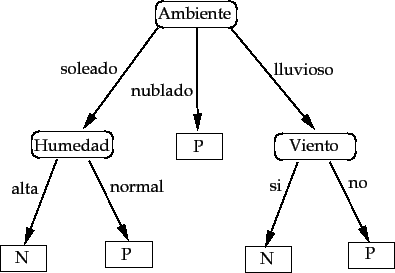
\includegraphics[width=0.7\linewidth]{capitulo-3/graphics/ad_1}
	\caption[Árbol de decisión]{Árbol de decisión}
	\label{fig:arbolEjemplo}
\end{figure}

En la figura por ejemplo un típico árbol de decisión que representa el concepto de jugar o no Golf, teniendo en cuenta variables climática representadas en los nodos internos, y los nodos hojas denotan las decisiones de jugar o no golf. 

\section{Algoritmo C4.5}
J.R Quinlan propone un mejora, una extensión al algoritmo ID3, al que denomina C4.5, este algoritmo genera un árbol de decisión a partir de los datos mediante particiones realizadas recursivamente. El árbol se construye mediante la estrategia profundidad-primero (depth-first).

El algoritmo C4.5 utiliza técnica heurística conocida como proporción de ganancia (gain-ratio). Es una medida basada en información que considera diferentes números y probabilidades de los resultados de las pruebas. 

El algoritmo considera todas las pruebas posibles que puede dividir el conjunto de datos, seleccionar la prueba que le haya generado mayor ganancia de información. Para cada atributo discreto, se considera una prueba con N resultados, siendo N el numero de valores posibles que puede tomar el atributo. Para cada atributo continuo, se realiza la prueba binaria (1,0) sobre cada uno de los valores que puede tomar el atributo de los datos.

\section{Características del algoritmo C4.5}
\begin{itemize}
	\item Permite trabaja con valores continuos para los atributos, separando los posibles resultados en dos ramas $ A_{i} <= N $ y $ A_{i} > N $ . 
	\item Los arboles son menos frondosos, ya que cada hoja cubre una distribución de clases no una clase en particular.
	\item Utiliza el método 'divide y vencerás' para generar el árbol de decisión incial a partir de un conjunto de datos de entrenamiento.
	\item Se basan en la utilización del criterio de proporción de ganancia, definido como $ I(X_{i},C) / I(X_{i})  $. De esta manera se consigue evitar que la variables con mayor numero de categorías salgan beneficiadas en la selección. 
	\item Es recursivo.
\end{itemize}

\section{Información de Ganancia / Entropía }
C4.5 como su predecesor ID3 utiliza la entropía como medida de selección para el atributo. 
Dado un nodo $N$ que representa las tuplas de la partición $D$. El atributo con mayor valor de ganancia es elegido para la división de $N$, el atributo reduce al mínimo la información necesaria para clasificar las tuplas de las particiones resultantes y refleja la menos aleatoriedad o impureza de la partición. Este enfoque minimiza el número esperado de los ensayos necesarios para clasificar una tupla dada y garantiza que un árbol simple (pero no necesariamente el más simple) se encuentre.

La información de ganancia necesaria para clasificar una tupla en $D$ es igual a:

\begin{equation}
Info(D) = - \displaystyle\sum_{i=1}^{m} p_{i}\log_2(p_{i}) 
\end{equation}

donde $p_{i}$ es la probabilidad de una tupla arbitraria en $D$ que pertenece a la clase $C_{i}$ se estima que es $ \lvert C_{i,D}} \rvert / \lvert D \rvert $. Se utiliza un logaritmo en base 2 porque la información esta codificada en bits. $Info(D)$ es la cantidad media de información necesaria para identificar la etiqueta de una tupla dada en $D$. Nótese, que la información que tenemos se basa solamente en las proporciones de tuplas de cada clase. $Info(D)$ también se conoce como entropía de $D$

Ahora, supongamos que estábamos para particionar las tuplas en $D$ en algunos atribuyen A teniendo $v$ valores distintos $ \{ a_{1},a_{2},...,a_{v} \}$, como se observa a partir de los datos de entrenamiento. Si A tiene valores discretos, estos valores se corresponden directamente con los resultados de una prueba de $v$ sobre $A$. El atributo $A$ se puede utilizar para dividir $D$ en $v$ particiones o subconjuntos, $ \{ D_{1},D_{2},...,D_{v} \}$, donde $D_j$ contiene aquellas tuplas en $D$ que tienen $a_j$ resultados de $A$. Estas particiones se corresponderían con las ramas que crecen a partir del nodo $N$. Idealmente, nos gustaría que esta división para producir una clasificación exacta de las tuplas. Es decir, nos gustaría para cada partición sea pura. Sin embargo, es bastante probable que las particiones sea impura (por ejemplo, cuando una partición puede contener una colección de tuplas de diferentes clases en lugar de una sola clase). ¿Cuánto más información sería todavía necesaria (después de la partición) con el fin de llegar a una clasificación exacta? Esta cantidad se mide por:

\begin{equation}
Info_{A}(D) = \displaystyle\sum_{j=1}^{v} \displaystyle\frac{\lvert D_{j} \rvert}{\lvert D \rvert} \times Info(D_{j})
\end{equation}

El termino $\displaystyle\frac{\lvert D_{j} \rvert}{\lvert D \rvert}$ actúa como el peso de la j-esima partición. $Info_{A}(D)$ es la información esperada requerida para clasificar la tupla de $D$ basada en la partición de $A$. Cuando menor sea la información esperada, mayor es la pureza de las particiones.

La información de ganancia se define como la diferencia entre lo requerido de información original (basado en la proporción de clases) y el nuevo requerimiento, obtenido luego de realizar la partición en $A$. Es decir,

\begin{equation}
Gain(A) = Info(D) - Info_{A}(D).
\end{equation}

En otras palabras, $Gain(A)$ nos dice cuanto se ganaría por la ramificación en $A$. Es la reducción esperada en el requisito de información causado por conocer el valor de $A$. El atributo A con ganancia mas alta, $Gain(A)$, se selecciona como atributo de división en el nodo $N$. Esto equivale a decir que queremos particionar en el atributo A que haría la mejor clasificación, por lo que la cantidad de información aun necesaria para clasificar las tuplas sea minima, $InfoA(D)$.


\section{Algoritmo}

\begin{algorithm}
	\caption{Árbol de Decisión - C4.5}
	\label{algoC45}
	\begin{algorithmic}[1]
		\Require Conjunto de datos etiquetados $D$
		\Procedure{C4.5}{$ D $}
			\If {$D > \textit{es puro o cumple el criterio de parada} $} 
				\State\textit{Termina}
			\EndIf
			\ForAll{$a \in D $}
				\State $\textit{Computar información de division en a }$
			\EndFor
			\State $ a_{best} =$ Mejor atributo de división respecto al criterio 
			\State $ Arbol =$ Crear un nodo de decisión con $ a_{best} $ en la raíz 
			\State $ D_{v} =$ Introducir sub-conjunto de $D$ basado en división $ a_{best} $
			\ForAll{$ D_{v} $}
				\State $ Arbol_{v} = C4.5(D_{v}) $
				\State Unir $ Arbol_{v} $ al correspondiente arco del Árbol
			\EndFor
			\State 
			\Return $ Arbol $
		\EndProcedure
	\end{algorithmic}
\end{algorithm}
     %Cap 3: Aprendizaje Automático
%Parte III: Desenvolvimiento

\chapter{Sistemas HAR móviles }

\label{chap4:sistemas-de-reconocimiento}

\section{Introducción}

\label{sec41:introduccion}El diseño de sistemas con conocimiento
del contexto promueven una interacción novedosa con los usuarios y
diversas aplicaciones en las áreas de ambientes inteligentes, repuesta
a emergencias, vigilancia y otros \cite{Choudhury2008}. Un sistema
con la capacidad de reconocer las actividades humanas por medio del
uso de sensores empotrados posee mecanismos para crear aplicaciones
de cuidado personal, salud y asistencia inteligente. El requerimiento
primordial de un sistema con una aplicación de contexto es que este
pueda ser portado continuamente como atuendo de sus usuarios (un sistema
\abbr{Wearable}). Por lo tanto, un sistema que acompaña continuamente
al usuario puede interaccionar oportunamente con el mismo ya que este
tiene la capacidad de observar en tiempo real las acciones de su portador.
La ventaja adicional de un sistema de este tipo es que puede ser desactivado
fácilmente o removido de la actividad diaria de su usuario.

En este capítulo se definen los componentes principales de un sistema
de reconocimiento de actividades humanas (sistemas \abbr{HAR}). El
objetivo principal del sistema \abbr{HAR} en conjunto es proveer
módulo base para aplicaciones novedosas de contexto. El módulo debe
ser capaz de reconocer varias actividades realizadas rutinariamente
de diferentes maneras, por diferentes usuarios y en diferentes condiciones
contextuales. Las funciones principales de los componentes descritos
en la primera sección exponen los mecanismos para implementar los
mismos en base trabajos relacionados de \abbr{HAR} \cite{Choudhury2008,ReyesOrtiz2015}. 

La última sección, enumera los requisitos no funcionales para lograr
una aplicación de contexto móvil y ubicua. Por un lado, las características
esperadas en una aplicación de esta naturaleza, y por el otro los
requisitos técnicos de los dispositivos móviles y los sensores empotrados
utilizados como instrumentos\footnote{\emph{hardware}} de implementación.

\section{Componentes}

\label{sec42:componentes}El diseño de la arquitectura de componentes
de un sistema \abbr{HAR} se rige de acuerdo a las guías de implementación
de una aplicación de aprendizaje automático (\abbr{ML}). De acuerdo
al proceso definido en la sección \ref{sec262:proceso-har}, se tiene
en cuenta la misma estructura de componentes y las mismas fases de
procesamiento de información. Además, se debe contemplar que el proceso
se divide en dos etapas: la etapa de entrenamiento y la de evaluación
\cite{LaraLabrador2013}. 

Ambas etapas requieren la implementación de los mismos componentes,
pero un sistema \abbr{HAR} práctico debe contemplar principalmente
la fase de evaluación, ya que el reconocimiento de actividades resulta
de una \emph{predicción} basado en un algoritmo de \abbr{ML} en-linea
(\emph{On-line learning}). Sin embargo, la etapa de entrenamiento
es un elemento clave para el sistema ya que es el punto de partida
para el \emph{aprendizaje} basado en modelo de \abbr{ML} y usualmente
se realiza bajo demanda (\emph{Off-line learning}).

Bajo el marco teórico de los sistemas \abbr{HAR} basados en \abbr{ML},
se han identificado unos componentes comunes para realizar las funcionalidades
de aprendizaje y predicción según \cite{Choudhury2008}. Un sistema
de reconocimiento de actividades posee tres componentes:
\begin{itemize}
\item un \emph{recolector }de medidas
\item un\emph{ procesador }de muestras 
\item un \emph{clasificador }de actividades
\end{itemize}
En la \figref{fig4:componentes-har} se muestra una vista general
de los componentes y sus interrelaciones. Las funcionalidades de cada
componente se describen a continuación. 

\begin{figure}[!tbph]
\centering{}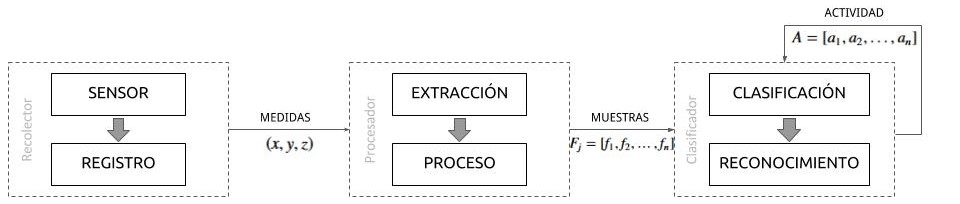
\includegraphics[width=1\linewidth]{capitulo-4/graphics/diagrama_4_1}\caption[Componentes \abbr{HAR}]{\label{fig4:componentes-har}Componentes de los sistemas \abbr{HAR}}
\end{figure}


\section{Recolector de medidas}

\label{sec43:recolector-datos}El primer paso en el proceso de reconocimiento
primeramente consiste en recolectar medidas de señales obtenidas de
los sensores que observan continuamente a los usuarios. Además, se
procede a realizar un registro de manera organizada e indexada con
respecto al tiempo. Para capturar los datos se requieren instrumentos
de medición apropiados como los sensores (\abbr{Wearables}, véase
\ref{sec23:sensores}). Los sensores capturan las señales directamente
de los usuarios por medio de observaciones continuas, al estar anexados
al cuerpo; en la cintura, la muñeca, el pectoral, los muslos o en
la cabeza \cite{Bao2004}. También, los sensores podrían ser portados
por el usuario ya están comúnmente empotrados en dispositivos de uso
regular como los teléfonos móviles modernos, en relojes o lentes inteligentes
\cite{LaraLabrador2012,Choudhury2008}.

A continuación se describe el método común de registro y organización
de los datos obtenidos de las señales continuas, además de algunos
ejemplos de variables relevantes utilizadas.

\subsection{Registro}

El método de registro consiste en capturar las señales de un sensor
y separar las medidas en una o más variables dependiendo del tipo
de sensor. La organización de los registros se realiza con respecto
al tiempo. Es decir, se dispone de un flujo continuo de datos con
una marca de tiempo almacenados de manera secuencial en un medio permanente
para su posterior procesamiento. 

La marca de tiempo usualmente se mide \emph{mili}-segundos y dependiendo
del sensor el intervalo entre medidas puede variar en el mismo orden,
Ej. con tasa de salida de \texttt{60 \abbr{Hz} }se tendrían 60 medidas
en un segundo. 

Las señales de sensores pueden clasificarse de la misma manera que
los grupos citados en la sección \ref{sec23:sensores}, según movimiento,
posición, entorno y fisiológicas. A continuación se describen en detalle
cada grupo.

\subsubsection{Señales de Movimiento}

Los sensores de movimiento proveen señales altamente informativos
para \abbr{HAR} debido a que miden las fuerzas de aceleración y rotación
en tres ejes cuando son portados por sus usuarios. En esta categoría
de sensores se encuentran los acelerómetros y giroscopios. 

Los acelerómetros miden señales de acuerdo a diferentes tipos de movimientos,
incluyendo la aceleración lineal y centrípeta, la gravedad y vibración
en dos o tres dimensiones \cite{Goehl2007}. Las variables medidas
están expresadas en la magnitud de la aceleración ejercida sobre el
dispositivo con respecto la orientación del mismo (Ej. en reposo mide
$-9.8\,m\,s^{-2}$ en dirección al suelo). La señal de la aceleración
dada por $a(t)$ es un vector con respecto al tiempo con tres componentes
en cada eje $(x,y,z)$, cada uno representa una medida $a_{x}$, $a_{y}$
y $a_{z}$. En la \figref{fig4:muestra-ac} se despliegan las medidas
obtenidas por la señal $a(t)$ durante una actividad física determinada.

\begin{figure}[!tbph]
\begin{centering}
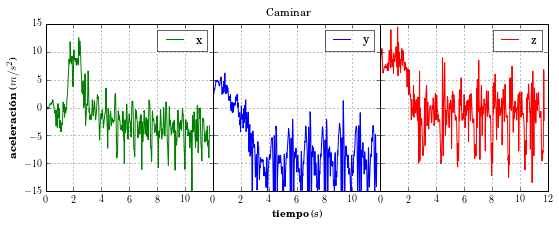
\includegraphics[width=1\columnwidth]{capitulo-4/graphics/signal_a3d}
\par\end{centering}
\caption[Señal de aceleración]{\label{fig4:muestra-ac}Señal de aceleración en tres dimensiones.
Los colores corresponden a los ejes de coordenadas representadas en
la siguiente figura.}
\end{figure}

Los giroscopios, o sensores de razón angular, miden señales de la
rapidez de rotación de los objetos en tres dimensiones \cite{Goehl2007}.
Las variables medidas están expresadas en velocidad angular de rotación
del dispositivo con respecto a los ejes de orientación del mismo (Ej.
en movimiento mide \foreignlanguage{english}{$-0.1\,rad\,s^{-1}$}
en relación a un eje fijo). La señal de la velocidad angular dada
por $w(t)$ es un vector con respecto al tiempo con tres componentes
en cada eje $(x,y,z)$, cada uno representa una medida $w_{x}$, $w_{y}$
y $w_{z}$. La orientación de los ejes con respecto al dispositivo
de medición depende del fabricante del mismo. Los teléfonos móviles
modernos poseen la orientación de los ejes de acuerdo a la siguiente
\figref{fig4:axis-phone}.

\begin{figure}[!tbph]
\begin{centering}
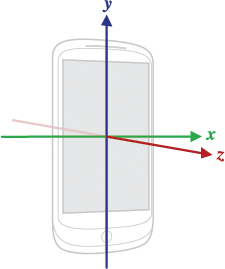
\includegraphics[scale=0.7]{capitulo-4/graphics/axis_device}
\par\end{centering}
\caption[Sistemas de coordenadas relativo a dispositivo]{\label{fig4:axis-phone}Ejes de coordenadas relativas a un teléfono
móvil moderno.}

\end{figure}

Las medidas obtenidas son variaciones con respecto a estos tres ejes
donde el valor $0$ está ubicado en el centro del dispositivo. Las
ventajas de los sensores de movimiento es su amplio uso al reconocer
actividades ambulatorias, como los citados en \cite{Bao2004,Kwapisz2011,ReyesOrtiz2015}.
Los acelerómetros y giroscopios poseen un bajo costo de fabricación,
bajo consumo de energía, y además están incluidos comúnmente en los
teléfonos móviles modernos \cite{Google2016s} debido a su utilidad
en mejorar la interacción humano-máquina por medio de gestos. Varios
trabajos publicados evidencian una alta precisión en \abbr{HAR} utilizando
al menos uno de estos sensores \cite{Bao2004,LaraLabrador2012}.

\subsubsection{Señales de Posición}

Los sensores de posición proveen señales con información adicional
que pueden ser utilizados para efectuar \abbr{HAR} y aplicaciones
de contexto con servicios basados en localización. En esta categoría
están los sensores de orientación (o brújula), magnetómetros y \abbr{GPS}
\cite{Google2016s}.

Las señales del \abbr{GPS} permiten acceder a las coordenadas geográficas
globales como el modo de transporte de un individuo, de acuerdo a
la velocidad estimada. Los teléfonos móviles modernos están equipados
con sensores para captar señales del sistema \abbr{GPS} y también
se puede estimar con buena precisión las coordenadas utilizando una
red celular \abbr{GSM}/\abbr{GPRS} y redes \abbr{WIFI} de corto
alcance. 

La señal de localización utiliza dos variables, conocidas como latitud
y longitud, y son medidas en la unidad radian (Ej. latitud $-57.2322\,rad$
y longitud $-25.3442\,rad$). Los valores de latitud y longitud son
coordenadas del \abbr{WGS} cuyos valores globales oscilan entre -180
a 180 en longitud, y -90 a 90 en latitud.

En la \figref{fig4:gps} se muestra una aplicación móvil para \abbr{Android}
que obtiene la estimación de coordenadas globales al triangular satélites
del \abbr{GPS}. 

\begin{figure}[!tbph]
\begin{centering}
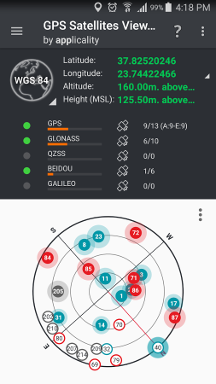
\includegraphics[scale=0.8]{capitulo-4/graphics/gps}
\par\end{centering}
\caption[Coordenadas por \abbr{GPS}.]{\label{fig4:gps}Visualización de satélites y coordenadas globales
basada en \abbr{GPS}.}
\end{figure}

Sin embargo, los \abbr{GPS} tienen cobertura limitada por la dificultad
de obtener señal dentro de edificaciones, o si no está disponible
servicio de red celular o \abbr{WIFI}. También el alto consumo de
energía es un factor importante si las aplicaciones rastrean la localización
en tiempo real. Además, la ubicación de un individuo es particularmente
información sensible para la mayoría de los usuarios y se debe tener
especial atención a no comprometer la privacidad de los datos y tener
el consentimiento del usuario para que este pueda ser rastreado \cite{LaraLabrador2013}.

\subsubsection{Señales del Ambiente}

Los sensores de ambiente solos no proveen información suficiente ya
que los individuos pueden realizar las actividades bajo diversas circunstancias
contextuales en términos de clima, ruido o iluminación. Por lo tanto
estos sensores pueden utilizarse de manera complementaria para detectar
sugestiones adicionales, Ej. el usuario está en el exterior de acuerdo
a la luminosidad, o se encuentra descansando debido a un nivel de
sonido y luminosidad baja \cite{LaraLabrador2013}.

Los sensores de ambiente miden varios atributos del entorno que rodea
al usuario. Algunas señales como la temperatura del aire, presión
atmosférica, iluminación, humedad, y el ruido pueden proveer información
de utilidad para conocer mejor el habitad particular de un usuario.
En esta categoría están los barómetros, fotómetros, termómetros y
micrófonos.

\subsubsection{Señales de Fisiológicas}

Los sensores fisiológicos proveen señales de signos vitales de un
individuo. La información sobre el ritmo cardíaco, tasa de respiración
y temperatura del cuerpo podrían ser combinados para enriquecer el
contexto durante el reconocimiento en ciertas aplicaciones específicas
como las orientadas a la salud \cite{LaraLabrador2013}.

\section{Procesador de muestras}

\label{sec44:proceso-se=0000F1ales}El siguiente paso en el reconocimiento
de actividades consiste en procesar las señales obtenidas por sensores
y extraer características relevantes de los datos en bruto. El modelo
de reconocimiento se construye a partir de un conjunto de muestras
etiquetadas utilizando métodos de aprendizaje automático en la etapa
de entrenamiento. Durante la etapa de evaluación las entradas con
las que un modelo construido opera son muestras no clasificadas pero
generadas con la misma técnica de muestreo utilizada durante el entrenamiento.

El procesador de muestras depende en tres tareas bien diferenciadas
que se realizan automáticamente en ambas etapas del proceso de reconocimiento,
adicionalmente se realiza una tarea manual durante la etapa de entrenamiento
llamada etiquetado. A continuación se detallan cada tarea.

\subsection{Etiquetado}

\label{ssec44:labeling}El proceso de aprendizaje automático requiere
de una cantidad moderada de datos recolectados a partir de usuarios
mientras realizan actividades humanas objetivas a nuestro estudio.
Estos datos deben ser recolectadas y etiquetados utilizando un teléfono
móvil inteligente con una aplicación diseñada para el caso, Ej. Utilizando
un teléfono con \abbr{Android} y la aplicación \emph{SensorLog} \cite{SLog2016}. 

El protocolo de recolección consiste en alistar un grupo de personas
que porten un teléfono inteligente mientras realizan con conjunto
específico de actividades y registrar datos por medio de la aplicación.
Las actividades de interés descritas en la sección \ref{sec263:actividades-humanas}
deben ser realizadas portando el teléfono en el bolsillo donde cada
individuo realiza una sesión de caminata, trote, bicicleta o conducir
un vehículo por un periodo de tiempo de 10 a 15 minutos. La recolección
de datos llevada a cabo por medio de la aplicación disponible para
la plataforma \abbr{Android} es mostrada en la \figref{fig4:sensor-log}. 

\begin{figure}[!tbph]
\begin{centering}
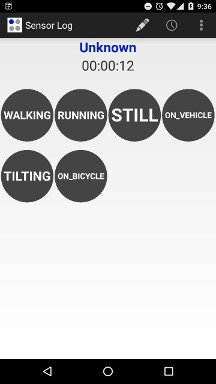
\includegraphics[scale=0.8]{capitulo-4/graphics/sensorlog1}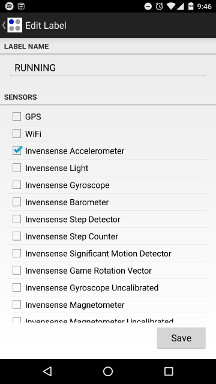
\includegraphics[scale=0.8]{capitulo-4/graphics/sensorlog2}
\par\end{centering}
\caption[Aplicación de entrenamiento SensorLog]{\label{fig4:sensor-log}Aplicación de entrenamiento \emph{SensorLog
}con interfaces de usuario para configurar y controlar la sesión de
entrenamiento}
\end{figure}

Así como se ve en la figura, la aplicación tiene una interfaz de usuario
simple que permite elegir los sensores de donde recolectar datos (Ej.
\abbr{GPS}, acelerómetro, giroscopio) para la sesión, las acciones
de iniciar y parar la actividad, y las etiquetas de la actividad que
el usuario realiza durante el entrenamiento. Las etiquetas utilizadas
en el proceso de recolección son:
\begin{itemize}
\item Caminar
\item Trotar
\item Quieto\footnote{A pesar de que esta actividad no representa un movimiento se incluye
como parte del estudio}
\item En bicicleta
\item En vehículo
\item \emph{Girando}\footnote{Esta no es una actividad física sino un comportamiento errático de
la orientación del teléfono}
\end{itemize}
La recolección se realiza obteniendo medidas a una razón de 60 a 100
\emph{mili}segundos por lo que se registran aproximadamente 60 a 100
muestras por segundo. Para asegurar la calidad de la recolección inicial
de datos las primeras sesiones de entrenamiento son supervisadas para
preparar las condiciones adecuadas del entrenamiento físico a elección
del participante.

\subsection{Filtro de Señal}

\label{ssec44:filtering}Teóricamente, si un dispositivo equipado
con sensores de movimiento está en reposo la señal de aceleración
$a(t)$ mediría cero (0) en dos ejes. Por ejemplo, en los ejes $x$
e $y$ no habría registro de medidas distintas a cero (0), y el eje
$z$mediría en dirección al suelo $-9.8\,m\,s^{-2}$. Sin embargo,
los sensores electrónicos pueden introducir cierta inestabilidad en
la señal (conocida como \emph{jitter}) provocando una fluctuación
en las lecturas debido a errores en la medición afectando la calidad
de los datos. Por lo tanto, a pesar de que un dispositivo con sensor
de movimiento esté completamente quieto en la mesa, las lecturas podrían
registrar ruido en los datos, Ej. errores del orden de $\pm0.005$. 

Entonces, para reducir ruido de la señal se debe aplicar uno o más
filtros. El filtro permite suavizar la señal por medio de una función
simple como la del cálculo de promedios variables (\emph{moving average})
o por un método como el de \emph{Butterworth} \cite{ReyesOrtiz2015}. 

Para el análisis de este trabajo se utilizó el filtro de señal de
promedios variables debido a su simplicidad y aplicabilidad basado
en otros trabajos como \cite{Yang2009}. El filtro de señal se puede
definir con la siguiente función $M$ descrita a continuación:

\label{def4:moving-average}\newtheorem{defs}{Definición}

\begin{defs}(\emph{Moving average}) Dada una secuencia $\left\{ a_{i}\right\} _{i=1}^{N}$,
un $n$-\emph{moving average} es una nueva secuencia $\left\{ s_{i}\right\} _{i=1}^{N-n+1}$
definida a partir de $a_{i}$ tomando la media aritmética de las \emph{sub}-secuencias
de tamaño $n$ donde,

\begin{eqnarray}
s_{i} & = & \frac{1}{n}\sum_{j=i}^{i+n-1}a_{j}
\end{eqnarray}

Así que las secuencias $S_{n}$ dado los $n$-\emph{moving averages}
serian 

\begin{eqnarray}
S_{2} & = & \frac{1}{2}(a_{1}+a_{2},a_{2}+a_{3},...,a_{n-1}+a_{n})
\end{eqnarray}

\begin{equation}
S_{3}=\frac{1}{3}(a_{1}+a_{2}+a_{3},a_{2}+a_{3}+a_{4},...,a_{n-2}+a_{n-1}+a_{n})
\end{equation}

y así sucesivamente.\end{defs}

Como ejemplo, en la \figref{fig4:filter-maf} se despliegan las gráficas
de una señal de aceleración $a_{y}$ para la dimensión $y$ y su correspondiente
señal filtrada con la función $M(a_{y})$ construida a partir de una
secuencia $S_{5}$ durante un intervalo de $1.6$ segundos. Como se
puede apreciar, la señal resultante está ligeramente suavizada debido
al filtrado de valores extremos resultado de perturbaciones bruscas
o ruido en la señal.

\begin{figure}[!tbph]
\begin{centering}
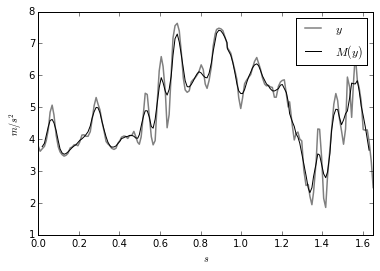
\includegraphics{capitulo-4/graphics/moving_average}
\par\end{centering}
\caption[Señal filtrada por la función $M$]{\label{fig4:filter-maf}Señal filtrada por promedios variables.}
\end{figure}


\subsection{Muestreo}

\label{ssec44:sampling}La realización de actividades humanas son
efectuadas durante periodos de tiempo de larga duración, en el orden
de los segundos o minutos. Esta taza es mucho mayor comparado con
las tazas de muestreos de los sensores, las cuales pueden llegar hasta
\texttt{250 \abbr{Hz}} (o \texttt{250} muestras por segundo). Una
simple medida capturada en un instante (Ej. la aceleración de $-2.5\,m\,s^{-2}$
en el eje $y$) no provee suficiente información para describir qué
actividad está llevando acabo un persona. Por lo tanto, las actividades
humanas deben ser reconocidas a partir de muestras extraídas en ventanas
de tiempo $w$ en vez de utilizar una sola medida instantánea en $t$. 

En la \tabref{tab4:ex-signal} se muestra una tabla con posibles medidas
instantáneas para la señal de aceleración $a(t)$ en una ventana de
tiempo $w_{j}$ con una taza de muestreo $r$asociada al sensor.

\begin{table}[!tbph]
\begin{centering}
\begin{tabular}{|c|c|c|c|c|}
\hline 
$w$ & $t$ & $a_{x}$ & $a_{y}$ & $a_{z}$\tabularnewline
\hline 
\hline 
$j$ & $0$ & \texttt{$1.3$} & \texttt{$-2.1$} & \texttt{$0$}\tabularnewline
\hline 
$j$ & $1/r$ & \texttt{$1.4$} & \texttt{$-2.3$} & \texttt{$0.1$}\tabularnewline
\hline 
$j$ & $2/r$ & \texttt{$1.1$} & \texttt{$-2.6$} & \texttt{$0$}\tabularnewline
\hline 
$j$ & $\ldots$ & \texttt{$\ldots$} & \texttt{$\ldots$} & \texttt{$\ldots$}\tabularnewline
\hline 
$j$ & $t_{max}$ & \texttt{$1.8$} & \texttt{$2.2$} & \texttt{$-0.4$}\tabularnewline
\hline 
\end{tabular}
\par\end{centering}
\caption[Medidas instantáneas de aceleración ]{\label{tab4:ex-signal}Ejemplo de medidas instantáneas de aceleración
en una ventana de tiempo.}
\end{table}

Las ventanas de tiempo hacen que las señales queden segmentadas en
muestras discretas utilizadas como unidades de reconocimiento de actividad.
De esta manera, cada ventana tiene inequívocamente una actividad humana
asociada y de esta manera podemos satisfacer el requisito planteado
por la definición del problema \ref{def2:harp-rel} en la sección
\ref{sec261:definicion-har}. 

Para incrementar la cantidad de muestras se utiliza una superposición
de $50\%$ con ventanas consecutivas y con tamaño de $2.56$ segundos,
como es recomendado por otros trabajos con técnicas de reconocimiento
\cite{Bao2004,ReyesOrtiz2015}. La superposición evita que ciertos
eventos se pierdan y las actividades se trunquen. La elección de este
tamaño de ventana produce muestras con medidas de tamaño fijo calculadas
aproximadamente con la ecuación \ref{eq4:window-size}. Este tamaño
es bastante conveniente por razones halladas en \cite{ReyesOrtiz2015}.

\begin{equation}
2.56\,\mathrm{sec}\times50\mathrm{\,Hz}=128\,\mathrm{medidas}\label{eq4:window-size}
\end{equation}

Cada muestra debe ser transformada en vectores característicos al
pasar por un proceso de extracción de valores que se describen en
la siguiente sección.

\subsection{Extracción}

\label{ssec44:extraction}Rememorando la definición del problema relajado\ref{def2:harp-rel}
en la sección \ref{sec261:definicion-har}, la incógnita principal
consiste en la comparación de las muestras provenientes de dos ventanas
$w_{1}$ y $w_{2}$, cada muestra con medidas $S_{j}$ que corresponden
a señales completamente distintas. Estas señales no serán idénticas
por más que sean obtenidas del mismo individuo realizando la misma
actividad física. Por lo tanto, para comparar muestras entres sí es
necesario extraer valores característicos en cada ventana $w_{j}$
por medio del filtro de información relevante y el calculo de valores
que identifiquen de cierta manera a las señales. 

El proceso de extracción se traduce en vectores característicos (\abbr{feature vectors})
con información relevante que componen varias métricas calculadas
en base a las ventanas $w_{j}$ en el dominio del tiempo. Las ventanas
son transformadas en el dominio de la frecuencia con métodos discretos
de\emph{ Fourier} utilizando algoritmos \abbr{FFT} con números reales. 

Los métodos de cálculo pueden ser de tipos estadísticos y estructurales
\cite{LaraLabrador2013} en base a lo propuesto por otros trabajos
precedentes como\cite{Yang2009,Bao2004}. Las métricas estadísticas
con respecto al tiempo y frecuencia utilizadas en este trabajo son:
\begin{enumerate}
\item \textbf{Media aritmética}: medida de tendencia central en la señal.
\item \textbf{Valor máximo}: medida de valor extremo en la señal.
\item \textbf{Valor mínimo}: medida de valor extremo en la señal.
\item \textbf{Desviación estándar}: media de dispersión en la señal.
\item \textbf{Energía}: promedio de suma de los cuadrados en la señal.
\item \textbf{Entropía}: (de Shannon) medida de incertidumbre utilizada
comúnmente en la Teoría de la Información aplicada a la señal en el
dominio de la frecuencia. Estima la cantidad de información en la
señal.
\item \textbf{Asimetría:} medida de distribución de simetría en el dominio
de la frecuencia.
\item \textbf{Curtosis:} medida de distribución de concentración en el dominio
de la frecuencia.
\item \textbf{Rango inter-cuartíl:}medida de dispersión de la diferencia
entre el tercer y primer cuartíl.
\item \textbf{Coeficientes autorregresivos:}los coeficientes obtenidos utilizando
el método de Burg que aplica un modelo autorregresivo para encajar
en la señal. La operación es aplicada a la señal en el dominio del
tiempo y produce cuatro (4) valores correspondientes al algoritmo
de 4to orden.
\item \textbf{Promedio en frecuencia:}medida de tendencia central en el
dominio de la frecuencia.
\end{enumerate}
En la \tabref{tab4:metricas} se resumen las métricas enumeradas anteriormente
en el orden establecido junto con el nombre de función y la formulación
matemática correspondiente para una señal dada$s$ en cualquier ventana$w_{j}$
de tamaño$n$.

\begin{table}[!tbph]
\begin{centering}
\begin{tabular}{|l|l|}
\hline 
Función & Formulación\tabularnewline
\hline 
\hline 
\texttt{mean(s)} & $\overline{s}=\frac{1}{n}\sum_{i=1}^{n}s_{i}$\tabularnewline
\hline 
\texttt{std(s)} & $\sigma=\sqrt{\frac{1}{n}\sum_{i=1}^{n}\left(s_{i}-\overline{s}\right)}$\tabularnewline
\hline 
\texttt{max(s)} & $\mathrm{max}(s)$\tabularnewline
\hline 
\texttt{min(s)} & $\mathrm{min}(s)$\tabularnewline
\hline 
\texttt{skewness(s)} & $\mathrm{E}\left[\left(\frac{s-\overline{s}}{\sigma}\right)^{3}\right]$\tabularnewline
\hline 
\texttt{kurtosis(s)} & $\frac{\mathrm{E}\left[\left(s-\overline{s}\right)^{4}\right]}{\mathrm{E}\left[\left(s-\overline{s}\right)^{2}\right]^{2}}$\tabularnewline
\hline 
\texttt{energy(s)} & $\frac{1}{n}\sum_{i=1}^{n}s_{i}^{2}$\tabularnewline
\hline 
\texttt{entropy(s)} & $s_{s}c_{i}=\sum_{i=1}^{n}c_{i}\log\left(c_{i}\right)\mathrm{\mathtt{\mathrm{,}}\,c_{i}}=s_{i}/\sum_{j=1}^{n}s_{j}$\tabularnewline
\hline 
\texttt{irq(s)} & $Q3(s)-Q1(s)$\tabularnewline
\hline 
\texttt{autoregression(s)} & $ar=\mathrm{arburg}\left(s,4\right)\mathrm{,}\,ar\in\mathbb{R}^{4}$\tabularnewline
\hline 
\texttt{meanFreq(s)} & $\sum_{i=1}^{n}\left(is_{i}\right)/\sum_{j=1}^{n}s_{j}$\tabularnewline
\hline 
\end{tabular}
\par\end{centering}
\caption[Métricas de valores característicos]{\label{tab4:metricas}Métricas para el calculo de vectores característicos
según\cite{ReyesOrtiz2015}.}
\end{table}

Las señales procesadas del conjunto $S$ corresponden al atributo
de la aceleración. Se utiliza un conjunto$S=\left\{ s_{0}\right\} $
con $k=1$, donde $s_{0}$ corresponde a la magnitud del vector resultante
de las medidas de fuerza ejercida en los tres ejes según la ecuación\ref{eq4:magnitud}.

\begin{equation}
\lVert a\rVert=\sqrt{a_{x}^{2}+a_{y}^{2}+a_{z}^{2}}\label{eq4:magnitud}
\end{equation}

Se eligió utilizar la magnitud $\lVert a\rVert$ del vector excluyendo
los valores unitarios en cada dimensión $a_{x}$,$a_{y}$,$a_{z}$
por los siguientes motivos:
\begin{itemize}
\item Simplicidad para utilizar la técnica de \abbr{DT}
\item Para cancelar el efecto de variaciones en la orientación del teléfono\cite{Schneider2014}
\item Reducir la dimensión de características (a un tercio) evitando sobre-ajustes
(\abbr{overfitting}).
\end{itemize}
El proceso de extracción transforma una ventana $w_{j}$ con señales
originales en un vector característico $F_{j}$ de dimensión $p$
como es representado en el ejemplo de la \tabref{tab4:features}.
Cada valor $\mathrm{f}_{0},\mathrm{f}_{1},\ldots,\mathrm{f}_{p}$
donde$p=14$ son obtenidos con una métrica particular enumerada anteriormente.

\begin{table}[!tbph]
\begin{centering}
\begin{tabular}{|c|c|c|c|}
\hline 
$w$ & $\mathrm{f}_{0}$ & $\ldots$ & $\mathrm{f}_{p}$\tabularnewline
\hline 
\hline 
$0$ & $2.71$ & \texttt{$\ldots$} & \texttt{$-2.30$}\tabularnewline
\hline 
$\ldots$ & $\ldots$ & \texttt{$\ldots$} & \texttt{$\ldots$}\tabularnewline
\hline 
$j$ & $2.91$ & \texttt{$\ldots$} & \texttt{$-4.11$}\tabularnewline
\hline 
$\ldots$ & $\ldots$ & \texttt{$\ldots$} & \texttt{$\ldots$}\tabularnewline
\hline 
$m-1$ & $2.56$ & \texttt{$\ldots$} & \texttt{$-5.56$}\tabularnewline
\hline 
\end{tabular}
\par\end{centering}
\caption[Métricas de proceso de extracción]{\label{tab4:features}Métricas procesadas a partir de las medidas
de señales}
\end{table}

Por último, se considera que tanto $S_{j}$ como $F_{j\ensuremath{}}$
tienen relación con al menos una etiqueta $\mathrm{a}_{k}$ particular
del conjunto $A$ ya sea debido a la función $f(S_{j})$ como resultado
de una evaluación, o como información en los datos del conjunto entrenamiento.

\section{Clasificador de actividades }

\label{sec45:clasificador}Un sistema \abbr{HAR} es similar a cualquier
aplicación de aprendizaje automático (\abbr{ML}) donde se requiere
de un algoritmo diseñado para extraer información desde los datos.
En este contexto los patrones son descubiertos a partir de un conjunto
de observaciones denominadas instancias \cite{LaraLabrador2013}.
El propósito principal del algoritmo es de clasificar los datos que
serán obtenidos a futuro. La entrada aplicada a un algoritmo de \abbr{ML}
es un conjunto de entrenamiento (\abbr{training set}) y el resultado
del mismo es un clasificador (\abbr{classifier}) \cite{Rajaraman2011}.
En esta sección se trata sobre clasificadores supervisados donde el
conjunto de entrenamiento incluye información acerca de la manera
correcta de clasificar un subconjunto de datos.

\subsubsection{Clasificación}

Es parte esencial de todo algoritmo de aprendizaje automático supervisado
contar con un conjunto de instancias de entrenamiento con información
adicional de clasificación. Cada instancia es un vector característico
$F_{j}$ calculado a partir de las señales $s$ contenidas en una
ventana de tiempo $w_{j}$. Como es requerido para todo clasificador
supervisado el conjunto de entrenamiento debe estar etiquetado con
una clase conocida así como se muestra en la tabla \tabref{tab4:labeled}.
La tarea de etiquetado debe ser realizada de forma manual como lo
citado en la sección \ref{ssec44:labeling}, o aunque difícil pero
no imposible manera automática.

\begin{table}[!tbph]
\begin{centering}
\begin{tabular}{|c|c|c|c|c|}
\hline 
$w$ & $\mathrm{f}_{0}$ & $\ldots$ & $\mathrm{f}_{m}$ & \emph{Actividad}\tabularnewline
\hline 
\hline 
$0$ & $2.71$ & \texttt{$\ldots$} & \texttt{$-2.30$} & \texttt{\small{}Desconocido}\tabularnewline
\hline 
$\ldots$ & $\ldots$ & \texttt{$\ldots$} & \texttt{$\ldots$} & \texttt{$\ldots$}\tabularnewline
\hline 
$j$ & $2.91$ & \texttt{$\ldots$} & \texttt{$-2.11$} & \texttt{\small{}Corriendo}\tabularnewline
\hline 
$\ldots$ & $\ldots$ & \texttt{$\ldots$} & \texttt{$\ldots$} & \texttt{$\ldots$}\tabularnewline
\hline 
$k-1$ & $2.56$ & \texttt{$\ldots$} & \texttt{$-2.56$} & \texttt{\small{}Caminando}\tabularnewline
\hline 
\end{tabular}
\par\end{centering}
\caption[Etiquetado de instancias]{\label{tab4:labeled}Etiquetado de instancias de entrenamiento}
\end{table}

A continuación se define formalmente el marco para algoritmos de aprendizaje
automático supervisados\cite{Rajaraman2011}.

\label{def4:clasificacion}\newtheorem{defs}{Definición}

\begin{defs}(Clasificador\abbr{ML}) Un algoritmo\abbr{ML} recibe
un conjunto entrenamiento se compone de varios pares $(\boldsymbol{x},y)$
conocidos como muestras de entrenamiento, donde
\begin{itemize}
\item $\boldsymbol{x}$ es un\emph{ vector} de valores, llamado vector característico.
\item $y$ es la\emph{ etiqueta}, el valor de clasificación para $\boldsymbol{x}$.
\end{itemize}
El objetivo del proceso\abbr{ML} es encontrar una función $y=f(\boldsymbol{x})$
cuya predicción de $y$ asociada a valores desconocidos de $\boldsymbol{x}$
sea la mejor. El valor de y corresponden a valores arbitrarios de
la siguiente naturaleza. Si $y$ es miembro de un conjunto finito
donde cada valor representa una clase particular. El problema es llamado
de clasificación de múltiples clases.\end{defs}

En el capítulo \ref{chap3:Aprendizaje-Automatico} se explica el algoritmo
C4.5 (sección \ref{sec3:algo-c45}) con enfoque basado en arboles
de decisión (\abbr{DT}) para construir la función $f$. La función
$f$ corresponde a un árbol de múltiples niveles donde cada nodo aplica
una función a $\boldsymbol{x}$ y determina sobre qué nodo hijo procede
la búsqueda. Cada nodo posee cualquier número de nodos hijos. Los
árboles de decisión son preferibles para las clasificación binaria
o de múltiples clases, especialmente cuando la dimensión del vector
característicos no es muy grande\cite{Rajaraman2011}.

\subsubsection{Reconocimiento}

Uno de los temas importantes acerca de los algoritmos de \abbr{ML}
es la manera en que los datos son tratados y utilizados para construir
un modelo de reconocimiento efectivo al clasificar datos desconocidos.
Al tratar con los datos, es una buena estrategia partir el conjunto
de entrenamiento (\abbr{training set}) disponible y separar un remanente
conocido como conjunto de validación (\abbr{test set}). El problema
de los algoritmos de \abbr{ML} es el sobre ajuste (\abbr{overfit}),
es decir, la clasificación resulta como se espera en el conjunto de
entrenamiento pero ante la mínima variación en datos desconocidos
de una población más grande el resultado es atípico o con errores
de clasificación \cite{Rajaraman2011}. Con este conjunto de validación
se puede evaluar el clasificador determinando si se sobre ajustan
los resultados.

\section{Capacidades deseables}

\subsection{Características no funcionales}

\label{ssec46:caracteristicas}Existen un conjunto de características
deseables que deben ser satisfechas para la construcción efectiva
de los sistemas de reconocimiento. Estas características abordan cuestiones
de diseño importantes que conciernen a la calidad y al funcionamiento
del sistema:
\begin{enumerate}
\item Portabilidad, el sistema utiliza sensores adjuntos a los individuos
(Ej. el acelerómetro) y no deben obstruir las actividades cotidianas
de los usuarios durante su uso. El fin es de evitar que se afecte
la adopción masiva del sistema. 
\item Conectividad, el sistema debe transmitir de manera confiable los datos
recolectados y/o procesados a algún componente desplegado de forma
remota. 
\item Almacenamiento, el sistema debe persistir los datos recolectados y/o
procesados de manera local en el dispositivo móvil con el fin de mantener
la calidad y minimizar la cantidad transferida a otros componentes.
\item Procesamiento, el sistema debe procesar y transformar los datos en
bruto para producir información relevante para el reconocimiento de
actividades.
\item Ubiquidad, el sistema debe operar en cualquier condición y contexto
en que la persona se encuentre sin interferir u obligar al usuario
a interactuar con el sistema.
\item Uso de energía, el sistema debe preservar el uso de energía en los
dispositivos móviles que están implementados. La lectura de datos,
el procesamiento y la conectividad no deben incurrir en gastos excesivos
de energía para que el sistema pueda operar.
\item Privacidad, el sistema debe mantener de manera confidencial los datos
recolectados y/o producidos durante la adopción masiva del sistema,
además de alertar sobre la utilización de datos sensibles que requieran
el consentimiento del usuario.
\end{enumerate}

\subsection{Dispositivos móviles}

\label{ssec46:dispositivos-moviles}Descripción técnica de dispositivos
móviles: procesador, memoria, sensores y almacenamiento

\subsubsection{Teléfonos móviles}

\subsubsection{Relojes inteligentes}

\subsection{Sensores empotrados}

\label{ssec46:sensores-empotrados}Descripción técnica de los sensores
de aceleración, variables, orientación en dispositivo, unidades de
medida, precisión vs consumo.

\subsubsection{Acelerómetro}

\subsubsection{Giroscopio}

\subsubsection{GPS/WIFI}

\section{Conclusión}

Resumen
 	%Cap 4: Sistemas HAR

\chapter{Sistemas de Reconocimiento de Actividades }

\label{chap:sistemas-de-reconocimiento}

Este capítulo describe la arquitectura común de un sistema de reconocimiento
de actividades. Se describe detalladamente los componentes del sistema
además de sus funciones principales de manera general. 

\section{Introducción}

Los sistemas de reconocimiento de actividades humanas son similares
a cualquier aplicación de aprendizaje automático. Según trabajos publicados
con anterioridad\cite{LaraLabrador2013}, los sistemas de reconocimiento
comparten una misma estructura de componentes y poseen las mismas
fases realizadas en dos etapas, entrenamiento y evaluación, así como
está descrito en el Capítulo 2 {[}ira al 2{]}. A pesar de que siguen
la misma guía de diseño puede que algunas implementaciones no incluyan
todos los componentes requeridos, es decir, un sistema puede implementar
simplemente los componentes necesarios para la etapa de evaluación
dejando de lado cualquier tarea en etapa de entrenamiento a realizarse
manualmente. 

\section{Componentes}

Actualmente, dentro del marco teórico del estudio de los sistemas
de reconocimiento, se han identificado unos componentes mínimos requeridos
para realizar las etapas de aprendizaje y predicción de manera automatizada\cite{choudhury2008mobile}.
Un sistema de reconocimiento de actividades posee tres componentes
o módulos principales que son:
\begin{itemize}
\item un \emph{módulo recolector de datos sensoriales} que recolecta toda
la información relevante para las actividades humanas utilizando por
supuesto sensores. Ej. el acelerómetro, giroscopio, brújula, etc.
\item un \emph{módulo de procesamiento y selección de muestras} que procesa
los datos en bruto para adecuarlos muestras con variables significativas
que permitan discriminar las actividades a reconocer
\item un \emph{módulo de clasificación }que utiliza las muestras extraídas
para inferir qué actividad probable está realizando un individuo en
un determinado instante.
\end{itemize}
Las responsabilidades y detalles de cada módulo se describen en los
siguientes apartados.

\subsection{Recolector de datos}

\subsection{Procesamiento y selección de muestras}

\subsection{Clasificación}

\section{Capacidades}

Existen un conjunto de características deseables que deben ser satisfechas
para la construcción efectiva de los sistemas de reconocimiento. Estas
características abordan cuestiones de diseño importantes que conciernen
a la calidad y al funcionamiento del sistema:
\begin{enumerate}
\item Portabilidad, el sistema utiliza sensores adjuntos a los individuos,
por ejemplo el sensor de aceleración, y no debe obstruir las actividades
cotidianas de una persona durante su uso para evitar que esto atente
contra la adopción masiva del sistema. 
\item Conectividad, el sistema debe poder transferir de manera confiable
los datos recolectados y procesados a un componente remoto. 
\item Almacenamiento, el sistema debe persistir datos recolectados y procesados
de manera local para mantener la calidad de los mismos y minimizar
la cantidad transferida a otro componente remoto.
\item Procesamiento, el sistema debe realizar tareas de procesamiento y
transformación de datos para producir información relacionada al reconocimiento
de actividades.
\item Ubiquidad, el sistema debe operar en cualquier condición y contexto
en que la persona se encuentre sin interferir u obligar a la persona
a interactuar con el sistema.
\item Uso de energía, el sistema debe preservar el uso de energía en los
dispositivos móviles que están implementados. La lectura de datos
de los sensores, el procesamiento y la conectividad no deben incurrir
en gastos excesivos de energía para que el sistema pueda operar.
\item Privacidad, el sistema debe de mantener de manera confidencial los
datos recolectados y producidos durante la adopción masiva del sistema,
además de avisar sobre la utilización de datos sensibles que puedan
requerir consentimiento del usuario.
\end{enumerate}

		%Cap 5: HARDroid: Un Sistema Reconocedor Colaborativo
%Parte IV: Resultados

\chapter{Evaluación y Resultados}

\label{chap6:evaluacion}

\section{Introducción}

En el ámbito de investigación y desarrollo de sistemas \abbr{HAR}
existen dos elementos vitales: la recolección de datos experimentales
y generación del conjunto de entrenamiento. En este capítulo, describimos
de manera general estos elementos en las primeras dos secciones. La
sección \ref{sec6:recoleccion} describe los aspectos relacionados
a la captura de datos, determinando los requisitos mínimos de los
teléfonos móviles utilizados y describiendo el procedimiento guía
para experimentación. Posteriormente, la sección \ref{sec6:clasificacion}
describe los resultados obtenidos al aplicar las técnicas descritas
en la sección \ref{sec44:proceso-se=0000F1ales} para transformar
datos sensoriales a un conjunto de entrenamiento para la clasificación
de actividades humanas. Finalmente, en la sección \ref{sec6:resultados}
los resultados producidos al utilizar el conjunto entrenamiento disponible
son presentados. Esto incluye la validación del modelo construido
con el algoritmo de \emph{Machine Learning} (\abbr{ML}) escogido
que confirma su usabilidad en ambientes productivos. También se expone
la evaluación de los resultados producidos por \emph{\abbr{HARDroid}
}con la aplicación \emph{ActivitySurvey} desarrollada para esta tarea.

\section{Datos Experimentales}

\label{sec6:recoleccion}En base a trabajos precedentes en sistemas
\abbr{HAR}, se han dispuesto datos experimentales para entrenar clasificadores
de actividades humanas tales como en \cite{ReyesOrtiz2013}. Estos
datos están disponibles como fuente para diversos estudios de investigaciones
en este ámbito. 

Sin embargo, los datos de sensores capturados con teléfonos móviles
son escasos. Es por esta razón que este trabajo requirió realizar
una colecta acorde a los objetivos de estudio del mismo. El procedimiento
y los datos recolectados por medio de experimentación se describen
a continuación.

\subsection{Instrumentación}

Como es sabido el desarrollo de \emph{\abbr{HARDroid} }se concreto
completamente para la plataforma \emph{\abbr{Android} }y a continuación
se detallan los rasgos técnicos de las herramientas utilizadas para
su concepción y evaluación.

\subsubsection{Teléfonos inteligentes}

Escoger las herramientas apropiadas para desarrollar un sistema \abbr{HAR}
requiere de la evaluación de dispositivos móviles disponibles en el
mercado teniendo en cuenta los criterios citados en la \secref{sec24:dispositivos-moviles}:
\emph{hardware}, sensores y software de plataforma. En el periodo
de evaluación de este trabajo (2016), la cantidad de teléfonos inteligentes
con sensores de aceleración fue vasta, algunos de los cuales se listan
en la \tabref{tab6:dispositivos} con sus características relevantes.

\begin{table}[h]
\begin{centering}
\begin{tabular}{|l|>{\raggedright}p{2.5cm}|l|>{\raggedright}p{2cm}|l|}
\hline 
Marca/modelo & CPU & RAM/ROM & Sensor & Android\tabularnewline
\hline 
\hline 
LG G2 & 1.2GHz Cortex-A7 & 1GB/8GB & BMI160 & Nougat 7.0\tabularnewline
\hline 
LG Nexus 5X & Q1.4Ghz Cortex-A53 & 2GB/32GB & BMC150 & Lollipop 5.0.2\tabularnewline
\hline 
Motorola G 2nd & 1.2GHz Cortex-A7 & 1GB/8GB & 3-axis Acc & Marshmallow 6.0\tabularnewline
\hline 
Huawei Mate 9 & Q2.4GHz Cortex-A73 & 4GB/64GB & LSM6DSM & Nougat 7.0\tabularnewline
\hline 
Huawei Mate 8 & Q2.3GHz Cortex-A72 & 3GB/32GB & LSM330  & Marshmallow 6.0\tabularnewline
\hline 
Samsung S6 & Q2.1GHz Cortex-A57 & 3GB/32GB & MPU6500 & Nougat 7.0\tabularnewline
\hline 
Samsung A5 & Q1.2GHz Cortex-A53  & 2GB/16GB & BOSCH & Lollipop 5.1.1\tabularnewline
\hline 
\end{tabular}
\par\end{centering}
\caption[Especificaciones de teléfonos inteligentes]{\label{tab6:dispositivos}Especificaciones de los teléfonos inteligentes
de entrenamiento.}
\end{table}

La elección fue en base a los dispositivos móviles disponibles, propiedad
de los voluntarios durante las diferentes sesiones de experimento.

\subsubsection{Entorno de desarrollo }

Las aplicaciones móviles desarrolladas en este trabajo están enteramente
construidas en la plataforma \emph{\abbr{Android}} donde fueron utilizados
los programas destinados para el caso \cite{Android2016}:
\begin{itemize}
\item \emph{Android Studio}: Entorno de desarrollo integrado para proyectos\emph{
}de software.
\item \emph{Android} \emph{Software Development Kit }(\abbr{SDK}): Herramientas
y librerías \abbr{API} requeridas para construir aplicaciones \emph{Android}.
\item \emph{Gradle}: Programa de automatización de tareas de construcción
de aplicaciones.
\end{itemize}
Las aplicaciones desarrolladas fueron escritas utilizando el lenguaje
\emph{Java }principalmente. Tanto las interfaces de usuario, servicios
de aplicación y las tareas de computación intensivas de acceso a sensores,
procesamiento, algoritmos de \abbr{ML} y almacenamiento de datos
fueron desarrollados integramente en \emph{Java}.

\subsection{Procedimiento Guía }

Con el objetivo de obtener un conjunto de datos adecuado a este estudio
de \abbr{HAR} se realizó un experimento de entrenamiento con grupo
de voluntarios. Un grupo de 8 personas entre las edades de 20 y 38
estuvieron dispuestos para esta tarea donde la edad media de la población
esta comprendida en $30.7\pm5$ años. 

El procedimiento guía de captura de datos se instruyó con el uso del
teléfono móvil como prenda sujeta al bolsillo o en la cintura mientras
se realiza una actividad física predeterminada. El planeamiento del
experimento consitió en realizar en orden por un periodo de 2 a 15
minutos alguna de las tres actividades básicas y dos de transporte.
Las actividades humanas con sus etiquetas correspondientes se listan
en la siguiente \tabref{tab6:etiquetas}.

\begin{table}[h]
\begin{centering}
\begin{tabular}[t]{|c|l|l|}
\hline 
Símbolo & Etiqueta & Descripción\tabularnewline
\hline 
\hline 
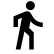
\includegraphics[scale=0.5]{capitulo-6/graphics/ic_activity_walk} & \emph{WALKING} & Caminar\tabularnewline
\hline 
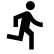
\includegraphics[scale=0.5]{capitulo-6/graphics/ic_activity_run} & \emph{RUNNING} & Trotar\tabularnewline
\hline 
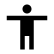
\includegraphics[scale=0.5]{capitulo-6/graphics/ic_activity_still} & \emph{STILL} & Estar quieto\tabularnewline
\hline 
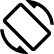
\includegraphics[scale=0.5]{capitulo-6/graphics/ic_activity_tilt} & \emph{TILTING} & Estar inquieto\tabularnewline
\hline 
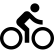
\includegraphics[scale=0.5]{capitulo-6/graphics/ic_activity_bike} & \emph{ON BICYCLE}  & Andar en bicicleta\tabularnewline
\hline 
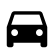
\includegraphics[scale=0.5]{capitulo-6/graphics/ic_activity_car} & \emph{IN VEHICLE}  & \multirow{1}{*}{Andar en automóvil}\tabularnewline
\hline 
\end{tabular}
\par\end{centering}
\caption{\label{tab6:etiquetas}Actividades humanas etiquetadas}
\end{table}

El resultado del experimento se resume en la \tabref{tab6:sesiones},
aquí se incluyen las sesiones hechas por los voluntarios y el tiempo
en minutos acumulado que fue invertido en cada actividad. 

\begin{table}[h]
\begin{centering}
\begin{tabular}{|c|c|c|c|c|c|c|}
\hline 
\multirow{2}{*}{Individuo} & \multicolumn{6}{c|}{Actividades}\tabularnewline
\cline{2-7} 
 & \emph{\footnotesize{}WALKING} & \emph{\footnotesize{}RUNNING} & \emph{\footnotesize{}STILL} & \emph{\footnotesize{}TILTING} & \emph{\footnotesize{}ON BICYLE} & \emph{\footnotesize{}IN VEHICLE}\tabularnewline
\hline 
\hline 
AG & 80 & 33 & 12 & 10 & 17 & 7\tabularnewline
\hline 
SG & 15 & 15 & - & - & - & -\tabularnewline
\hline 
SF & 43 & 25 & - & - & 13 & -\tabularnewline
\hline 
GA & 30 & 2 & - & - & - & -\tabularnewline
\hline 
BV & - & 17 & - & - & - & -\tabularnewline
\hline 
PV & 17 & 19 & 12 & - & - & 7\tabularnewline
\hline 
SY & 37 & 13 &  & 10 & 26 & 11\tabularnewline
\hline 
MD & 29 & 4 & - & - & - & -\tabularnewline
\hline 
\end{tabular}
\par\end{centering}
\caption{\label{tab6:sesiones}Resumen de sesiones de entrenamiento}
\end{table}


\subsection{Captura de Datos}

El experimento requiere de una cantidad de datos recolectados de los
voluntarios mientras realizan las actividades humanas dictadas durante
el entrenamiento. \emph{SensorLog} \cite{Alan2014s} es una aplicación
\abbr{Android} que se utilizó para la captura y persistencia de las
señales del sensor de aceleración como se ve en la \figref{fig4:sensor-log}.
La aplicación permite exportar las señales de sensores almacenadas
en forma agrupada por sesiones y subirlas a la nube. En la \tabref{tab6:captura}
se resumen las cantidades de medidas de señales capturadas.

\begin{table}[h]
\begin{centering}
\begin{tabular}{|c|c|c|c|c|c|}
\hline 
\multicolumn{6}{|c|}{Actividades}\tabularnewline
\hline 
\emph{\footnotesize{}WALKING} & \emph{\footnotesize{}RUNNING} & \emph{\footnotesize{}STILL} & \emph{\footnotesize{}TILTING} & \emph{\footnotesize{}ON BICYLE} & \emph{\footnotesize{}IN VEHICLE}\tabularnewline
\hline 
\hline 
3.591.788 & 1.604.270 & 387.735 & 134.566 & 819.992 & 365.814\tabularnewline
\hline 
\end{tabular}
\par\end{centering}
\caption{\label{tab6:captura}Unidades de datos capturados}
\end{table}


\subsection{Conjunto de Entrenamiento }

En la \tabref{tab6:muestras} se resumen las cantidades de las muestras
calculadas de acuerdo lo descrito en el proceso de la \secref{ssec44:extraction}.

\begin{table}[h]
\begin{centering}
\begin{tabular}{|c|c|c|c|c|c|}
\hline 
\multicolumn{6}{|c|}{Actividades}\tabularnewline
\hline 
\emph{\footnotesize{}WALKING} & \emph{\footnotesize{}RUNNING} & \emph{\footnotesize{}STILL} & \emph{\footnotesize{}TILTING} & \emph{\footnotesize{}ON BICYLE} & \emph{\footnotesize{}IN VEHICLE}\tabularnewline
\hline 
\hline 
5.915 & 3.019 & 645 & 485 & 1.338 & 610\tabularnewline
\hline 
\end{tabular}
\par\end{centering}
\caption{\label{tab6:muestras}Unidades de muestras procesadas}
\end{table}

El proceso de generación del clasificador está automatizado por medio
del flujo mostrado en la \figref{fig6:proceso-clasi}.

\begin{figure}[th]
\begin{centering}
\includegraphics[width=0.8\textwidth]{\string"capitulo-6/graphics/Proceso de Clasificacion\string".png}
\par\end{centering}
\caption{\label{fig6:proceso-clasi}Flujo de generación del clasificador C4.5}
\end{figure}


\section{Clasificador de Actividades Humanas}

\label{sec6:clasificacion}Un clasificador de actividades humanas
es un clasificador de clases discretas que utiliza un algoritmo de
aprendizaje automático supervisado basado en árboles de decisión.
Este clasificador evalúa como entrada una instancia sin etiquetar
obtenida a partir de datos observados y produce como salida una predicción
de la etiqueta más probable asociada en base a observaciones previas.

En esta sección se describe el procedimiento de generación de un clasificador
\abbr{HAR} utilizando un conjunto de entrenamiento inicial. Luego
se evalúa el mismo por medio de pruebas y verificación para garantizar
su efectividad. Este procedimiento se realiza utilizando la herramienta
de aprendizaje automático denominado \emph{Waikato Environment Knowledge
Analysis} \texttt{(\abbr{WEKA})} \cite{Frank2016}. 

\subsection{Métricas de predicción numérica}

De manera a evaluar el rendimiento de los clasificadores de aprendizaje
automático supervisado se describen las siguientes medidas y métricas
de predicción numéricas que dan una noción de cuánto se acercan las
predicciones a los datos observados \cite{Witten2017}.

Utilizando la siguiente nomenclatura de la definición \ref{def3:clasificacion}
de la \secref{sec3:aprendizaje} en que $\hat{f}(x_{i})$ corresponde
a los valores de la predicción de una instancia de evaluación $x_{i}$
e $y_{i}$ corresponde al valor actual de la \emph{$i$-ésima} instancia,
se define cuanto sigue:
\begin{itemize}
\item \emph{Número de instancias}: es el tamaño de la población de entrada
$N$.
\item \emph{Instancias correctamente clasificadas}: es una proporción del
tamaño de la población de entrada $C$.
\item \emph{Instancias incorrectamente clasificadas}: es un proporción del
tamaño de la población de entrada $I$.
\item \emph{Estadísticas Kappa}: es el coeficiente \emph{kappa} de \emph{Cohen}
que establece el valor de coeficiente de concordancia para confiabilidad
de los datos. 
\[
\kappa\text{=}\frac{p_{o}-p_{e}}{1-p_{e}}
\]
, donde $p_{o}$ es el acuerdo observado relativo y $p_{e}$ es la
probabilidad hipotética de acuerdo. Los valores se dividen en los
siguientes rangos.\\
\\
\begin{tabular}{|c|c|c|}
\hline 
Valor & Nivel de acuerdo & \% de datos confiables\tabularnewline
\hline 
\hline 
0 - 0.20 & No & 0 - 4\%\tabularnewline
\hline 
0.21 - 0.39 & Mínimo & 4 - 15\%\tabularnewline
\hline 
0.40 - 0.59 & Débil & 15 - 35\%\tabularnewline
\hline 
0.60 - 0.79 & Moderado & 35 - 63\%\tabularnewline
\hline 
0.80 - 0.90 & Fuerte & 64 - 81\%\tabularnewline
\hline 
>0.90 & Casi perfecto & 82 - 100\%\tabularnewline
\hline 
\end{tabular}
\item \emph{Error medio absoluto}: es el promedio de la magnitud de los
errores absolutos individuales.
\[
\frac{1}{n}\sum_{i\text{=1}}^{n}\bigl|y_{i}-\hat{f}(x_{i})\bigr|
\]
\item \emph{Raíz de Error cuadrático medio}: es la raíz del promedio de
la magnitud de los errores individuales elevados al cuadrado.
\[
\sqrt{\frac{1}{n}\sum_{i\text{=1}}^{n}\left(y_{i}-\hat{f}(x_{i})\right)^{2}}
\]
\item \emph{Error absoluto relativo}: es la razón de la suma de los errores
absolutos y la suma de las diferencia absoluta de los valores exactos
con la media. 
\[
\sum_{i\text{=1}}^{n}\frac{\bigl|y_{i}-\hat{f}(x_{i})\bigr|}{\bigl|y_{i}-\bar{y}\bigr|}\,\textrm{, donde\,}\bar{y}=\frac{1}{n}\sum_{i=1}^{n}y_{i}
\]
\item \emph{Raíz de Error cuadrático relativo}: es la raíz de la razón de
la suma de los errores individuales elevados al cuadrado y la suma
de las diferencia de los valores exactos con la media elevados al
cuadrado. 
\[
\sqrt{\sum_{i\text{=1}}^{n}\frac{\left(y-\hat{f}(x_{i})\right)^{2}}{\left(y_{i}-\bar{y_{i}}\right)^{2}}}
\]
\end{itemize}

\subsection{Evaluación del clasificador}

El clasificador generado en este trabajo es un árbol de decisión obtenido
por medio del algoritmo C4.5 (\algref{algoC45}) y la implementación
en \emph{Java} J48 \cite{Frank2016b}. El tamaño del árbol generado
es de $677$ nodos, de los cuales $339$ corresponden a hojas.

A continuación se presentan las métricas numéricas de predicción del
clasificador generado con las muestras de entrenamiento recolectadas
y descritas anteriormente: 
\begin{itemize}
\item Número de instancias: $12.012$ 
\item Instancias correctamente clasificadas: $10.942$ (en porcentaje $91,0922$
\%)
\item Instancias incorrectamente clasificadas: $1.070$ (en porcentaje $8,9078$
\%)
\item Estadísticas Kappa: $0,8678$ 
\item Error medio absoluto: $0,0341$
\item Raíz de Error cuadrático medio: $0,164$ 
\item Error absoluto relativo: $15,1717$ \% 
\item Raíz de Error cuadrático relativo: $48,9126$ \% 
\end{itemize}
En general, se puede apreciar que la taza de errorres es baja, la
cantidad de instancias correctas alta y el coeficiente de confianza
es fuerte. Adicionalmente, en la \tabref{tab6:matriz-confusion} se
muestra la matriz de confusión obtenida así como se detalla en la
\secref{sec3:metricas}. 

\begin{table}[h]
\begin{centering}
\begin{tabular}{|l|c|c|c|c|c|c|}
\cline{2-7} 
\multicolumn{1}{l|}{} & \multicolumn{6}{c|}{Matriz de Confusión}\tabularnewline
\hline 
Actividad & \emph{\footnotesize{}WALKING} & \emph{\footnotesize{}RUNNING} & \emph{\footnotesize{}STILL} & \emph{\footnotesize{}TILTING} & \emph{\footnotesize{}ON BICYLE} & \emph{\footnotesize{}IN VEHICLE}\tabularnewline
\hline 
\hline 
\emph{\footnotesize{}WALKING} & 5.643 & 63 & 21 & 28 & 156 & 4\tabularnewline
\hline 
\emph{\footnotesize{}RUNNING} & 122 & 2.852 & 3 & 6 & 36 & 0\tabularnewline
\hline 
\emph{\footnotesize{}STILL} & 19 & 14 & 555 & 23 & 15 & 19\tabularnewline
\hline 
\emph{\footnotesize{}TILTING} & 26 & 3 & 21 & 304 & 46 & 85\tabularnewline
\hline 
\emph{\footnotesize{}ON BICYLE} & 157 & 28 & 7 & 47 & 1.089 & 10\tabularnewline
\hline 
\emph{\footnotesize{}IN VEHICLE} & 2 & 2 & 14 & 86 & 7 & 499\tabularnewline
\hline 
\end{tabular}
\par\end{centering}
\caption{\label{tab6:matriz-confusion}Matriz de confusión del clasificador
resultante}
\end{table}

A partir de esta matriz se obtuvieron los siguientes calculos de métricas
de evaluación para clasificadores expuesto también en la \secref{sec3:metricas}:
\begin{itemize}
\item Precisión: $0,9174$
\item Exhaustividad: $0,9109$
\item Exactitud: $0,9714$
\item \emph{Valor-F}: $0,9142$
\end{itemize}
Finalmente, se puede apreciar que los valores demuestran una buena
efectividad del clasificador generado debido a que las métricas están
por encima de 90\%.

\section{Resultados Experimentales}

\label{sec6:resultados}En esta sección se describen los resultados
del experimento realizado utilizando la aplicación \emph{ActivitySurvey}
que utiliza el reconocedor \emph{HARDroid}, ambos desarrollados en
este trabajo. Los datos presentados en esta sección permiten verificar
la correctitud de los componentes de software implementados así como
también validar las predicciones emitidas por el reconocedor de actividades
humanas contribuido en este trabajo.

\subsection{Verificación del clasificador}

Para verificar el clasificador de \emph{HARDroid }se condujo un experimento
de prueba basado en una sesión de actividades físicas realizadas por
dos personas. El protocolo consitió en realizar cada una de las actividades
básicas ambulatorias y de transporte por un periodo comprendido entre
10 a 20 minutos utilizando la aplicación \emph{ActivitySurvey}. 

En la \tabref{tab6:vsesiones} se resume el tiempo en minutos invertido
por cada persona en las actividades realizadas en un lapso de una
hora aproximadamente.

\begin{table}[th]
\begin{centering}
\begin{tabular}{|c|c|c|c|c|c|c|}
\hline 
\multirow{2}{*}{Individuo} & \multicolumn{6}{c|}{Actividades}\tabularnewline
\cline{2-7} 
 & \emph{\footnotesize{}WALKING} & \emph{\footnotesize{}RUNNING} & \emph{\footnotesize{}STILL} & \emph{\footnotesize{}TILTING} & \emph{\footnotesize{}ON BICYLE} & \emph{\footnotesize{}IN VEHICLE}\tabularnewline
\hline 
\hline 
nexus5x & 14 & 10 & 10 & - & 20 & 14\tabularnewline
\hline 
mate9 & 12 & 7 & 18 & - & 15 & 14\tabularnewline
\hline 
\end{tabular}
\par\end{centering}
\caption{\label{tab6:vsesiones}Resumen de sesiones de evaluación}
\end{table}

La aplicación \emph{ActivitySurvey} registra durante la sesión de
evaluación los datos del individuo, la fecha y hora de la actividad
detectada y la etiqueta de actividad aseverada en caso de una predicción
correcta o una corrección de la etiqueta real. 

En la \tabref{tab6:vencuesta} se resumen las cantidades de actividades
detectadas correcta e incorrectamente en proporción con el total a
partir de la encuesta realizada durante cada sesión. La respuesta
incorrecta corresponde a una etiqueta obtenida por retro alimentación
del usuario.

\begin{table}[h]
\begin{centering}
\begin{tabular}{|l|c|c|c|c|c|c|}
\cline{2-5} 
\multicolumn{1}{l|}{} & \multicolumn{4}{c|}{\textbf{Incorrecta}} & \multicolumn{1}{c}{} & \multicolumn{1}{c}{}\tabularnewline
\hline 
Actividad & \emph{\footnotesize{}WALKING} & \emph{\footnotesize{}STILL} & \emph{\footnotesize{}ON BICYLE} & \emph{\footnotesize{}IN VEHICLE} & \textbf{\small{}Correcta} & \textbf{\small{}Porcentaje}\tabularnewline
\hline 
\hline 
\emph{\footnotesize{}WALKING} &  &  & 13 &  & 145 & 91,77\%\tabularnewline
\hline 
\emph{\footnotesize{}RUNNING} &  &  & 13 &  & 83 & 86,46\%\tabularnewline
\hline 
\emph{\footnotesize{}STILL} &  &  &  & 8 & 140 & 94,59\%\tabularnewline
\hline 
\emph{\footnotesize{}TILTING} &  &  &  & 38 & 0 & 0,00\%\tabularnewline
\hline 
\emph{\footnotesize{}ON BICYLE} & 18 &  &  & 14 & 59 & 64,84\%\tabularnewline
\hline 
\emph{\footnotesize{}IN VEHICLE} &  & 11 &  &  & 83 & 88,30\%\tabularnewline
\hline 
\end{tabular}
\par\end{centering}
\caption[Actividades correctas e incorrectas]{\label{tab6:vencuesta}Resumen de actividades detectadas correctas
e incorrectas}
\end{table}


\subsection{Validación de la clasificación}

Para validar los resultados de la clasificación de \emph{HARDroid
}se condujo un experimento de prueba basado en la misma sesión de
actividades físicas realizadas por una persona. El protocolo consitió
en utilizar la aplicación \emph{Sony} \emph{LifeLog} a la par de la
aplicación \emph{ActivitySurvey} durante las sesiones de evaluación. 

En la \tabref{tab6:vclasificacion} se muestra el tiempo invertido
en minutos en cada actividad humana realizado por una persona.

\begin{table}[h]
\begin{centering}
\begin{tabular}{|c|>{\raggedright}p{3cm}|c|c|>{\raggedright}p{3cm}|c|}
\hline 
Sesión & Actividad \emph{LifeLog} & Intervalo & Duración & Actividad \emph{HARDroid} & Razón\tabularnewline
\hline 
\hline 
nexus5x & walking & 21:26 - 21:44 & 19 & WALKING & 45/9\tabularnewline
\hline 
nexus5x & cycling & 21:44 - 22:00 & 27 & ON\_BICYCLE & 32/18\tabularnewline
\hline 
nexus5x & running & 22:12 - 22:24 & 13 & RUNNING & 41/0\tabularnewline
\hline 
nexus5x & vehicle & 22:39 - 22:57 & 19 & IN\_VEHICLE & 32/6\tabularnewline
\hline 
nexus5x & - & 22:25 - 22:35 & 10 & STILL & 65/0\tabularnewline
\hline 
\end{tabular}
\par\end{centering}
\caption[Evaluación \emph{HARDroid} vs \emph{Sony LifeLog}]{\label{tab6:vclasificacion}Resumen de actividades detectadas \emph{HARDroid}
vs\emph{ Sony LifeLog}}
\end{table}

Cada actividad detectada por \emph{HARDroid} es validada con la aplicación
\emph{Sony} \emph{LifeLog} y además se inclyye la razón de correctas
versus incorrectas. En la \figref{fig6:vlifelog} se muestra la salida
de la aplicación \emph{Sony Lifelog }de la sesión individual.

\begin{figure}
\begin{centering}
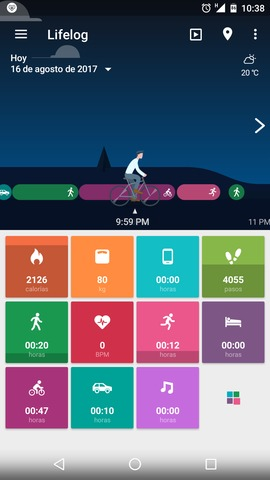
\includegraphics[scale=0.7]{capitulo-6/graphics/lifelog1} 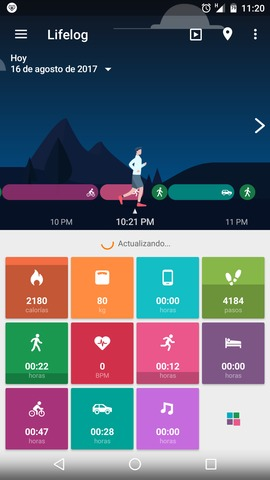
\includegraphics[scale=0.7]{capitulo-6/graphics/lifelog2}
\par\end{centering}
\caption[Evaluación con aplicación \emph{Sony Lifelog}]{\label{fig6:vlifelog}Resultado de sesión de evaluación con \emph{Sony
Lifelog}}

\end{figure}

		%Cap 6: Evaluación
%Parte V: Final

\chapter{Conclusiones y Trabajos Futuros}

\label{cap8:conclusiones-y-trabajos-futuros}

\section{Conclusiones del presente trabajo}

\label{sec81:conclusiones}El reconocimiento de actividades humanas
es un área de investigación multidisciplinaria con constantes aportes
y diversos usos en la actualidad debido a su relevancia en la computación
contextual y ubicua. Los avances en la miniaturización de los sistemas
de computación y sensores hacen del área un tanto atractiva como desafiante
para explorar y proponer nuevas ideas en este ámbito \cite{LaraLabrador2013}. 

Los esfuerzos realizados en este trabajo han tenido en cuenta además
la colaboración y el uso de Internet de manera a aprovechar los mismos
en la mejora de los sistemas de reconocimiento, y como se mostró en
la sección anterior la aplicación de resultados colaborativos puede
ser aprovechada para mejorar el sistema desarrollado. 

Así, en este trabajo se construyó un sistema de reconocimiento de
actividades colaborativo que utiliza tres elementos principales: teléfonos
móviles inteligentes, una librería que a la par se ha hecho disponible
como software libre y la Internet. 

El desarrollo del trabajo se llevó acabo en dos etapas. La primera
etapa consistió en el entrenamiento de un clasificador y la segunda
etapa consistió en la construcción de un sistema reconocedor de actividades
para teléfonos móviles. Los principales aportes de este trabajo se
produjeron en la segunda etapa:
\begin{itemize}
\item Por una parte se tiene como resultado tangible un componente de código
abierto reutilizable para reconocer actividades humanas. Este componente
es denominado \emph{HARDroid}.
\item Por otra parte este componente posibilita el mejoramiento iterativo
de su desempeño mediante un esquema colaborativo.
\end{itemize}
Respecto al primer punto, es importante destacar que \emph{HARDroid}
puede ser aprovechado por otras aplicaciones móviles de dos maneras
concretas \cite{GimenezYegros2016a}: 
\begin{itemize}
\item el mismo puede ser incluido en tiempo de construcción, o
\item puede ser aprovechado como un servicio a través de una interfaz de
integración.
\end{itemize}
Los experimentos realizados en el presente trabajo y documentados
en la sección previa muestran que \emph{HARDroid} es capaz de producir
un modelo en el cual se observan las siguientes características:
\begin{itemize}
\item Una alta tasa de aciertos ($91$\% a $92$\%), y por lo tanto una
baja tasa de errores. Esto se puede verificar en la MATRIZ DE CONFUSION
RESULTANTES
\item La capacidad de extender el modelo para reconocer diversos tipos de
actividades como, en bicicleta, en vehículo, entre otros.
\item La posibilidad colaborativamente el modelo mediante la inclusión de
muestras de aciertos colectadas en campo.
\end{itemize}
(REVISAR CONCLUSIONES COMPLEMENTANDO CON REF A LOS RESULTADOS)

\section{Trabajos Futuros propuestos}

\label{sec82:trabajos-futuros}Luego de la experiencia obtenida y
documentada en el presente trabajo, teniendo en cuenta la amplia aplicabilidad
del reconocimiento de actividades humanas en especial en aplicaciones
para dispositivos móviles, a continuación se proponen algunos trabajos
que se desprenden del presente:
\begin{enumerate}
\item Segmentar los grupos de individuos distintos por rangos de edad, sexo
y/o factores fisiológicos y otros, de manera a generar modelos específicos
para cada grupo que posibiliten el desarrollo de una nueva gama de
aplicaciones. 
\item Incorporar al sistema \emph{HARDroid} desarrollado otros métodos de
aprendizaje automático que permitan mejorar la tasa de aciertos. Entre
estos se sugieren por ejemplo las técnicas de vectores de soporte
(\abbr{SVM}) o redes neuronales (\abbr{ANN}).
\item Incluir más variables en el procesamiento de señales de entrada para
mejorar las predicciones teniendo en cuenta la orientación del dispositivo. 
\item Extender el sistema \emph{HARDroid} para identificar otras actividades
humanas aplicado a otras disciplinas o contextos. Por ejemplo en medicina
para detectar caídas, posturas o actividades no recomendadas. En el
campo militar para recomendar actividades más favorables para situación.
\item Utilizar o aprovechar otros accesorios que agreguen variables relevantes
en el reconocimiento de actividades dependiendo del contexto. Por
ejemplo, un reloj inteligente (\emph{\abbr{Smartwatch}}).
\end{enumerate}

		%Cap 7: Conclusiones y Trabajos Futuros

\appendix   
% los capítulos que incluyas a partir de aquí aparecen
% como apendices
\colorlet{punct}{red!50!black}
\definecolor{background}{HTML}{F3F6FF}
\definecolor{delim}{RGB}{20,105,176}
\colorlet{numb}{magenta!50!black}

\lstdefinelanguage{json}{
	basicstyle=\tiny\ttfamily,
	numberstyle=\scriptsize,
	stepnumber=1,
	numbersep=4pt,
	showstringspaces=false,
	breaklines=true,
	frame=lines,
	backgroundcolor=\color{background},
	literate=
	*{:}{{{\color{punct}{:}}}}{1}
	{,}{{{\color{punct}{,}}}}{1}
	{\{}{{{\color{delim}{\{}}}}{1}
	{\}}{{{\color{delim}{\}}}}}{1}
	{[}{{{\color{delim}{[}}}}{1}
	{]}{{{\color{delim}{]}}}}{1},
}


\chapter{Sincronización de Resultados}

\label{chapA:rest-api}

En este anexo, se proporcionan detalles adicionales los servicios REST para realizar, incluyendo ejemplos y relación entre los recursos.

El servicio se comprende de dos recursos \textit{Collaborativefeature} y \textit{Collaborativesession}, el primero de estos representa la colección de los 15 feature calculados de una ventana de tiempo, y por otro lado la session de una actividad realizada por el individuo, la cual incluye una lista de features, como se esquematiza en la siguiente figura \ref{fig:der} .

\begin{figure}[!htbp]
	\centering
	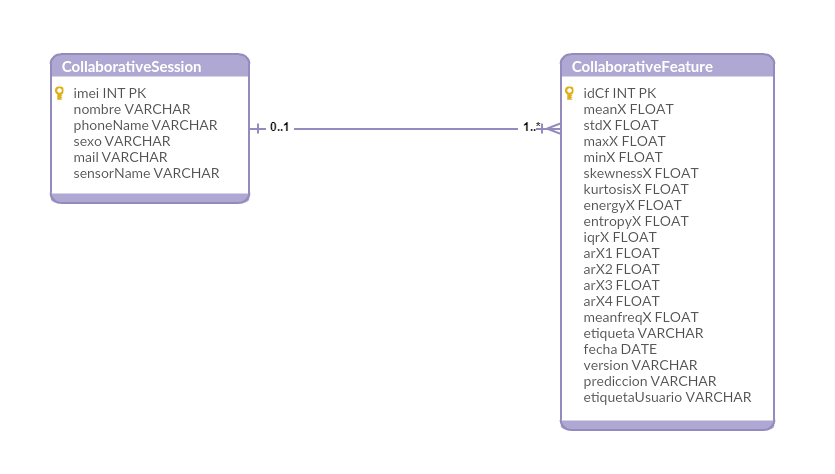
\includegraphics[width=0.7\linewidth]{anexos/der}
	\caption[Modelo de Datos]{\label{fig:der}Modelo de Datos}
\end{figure}

Los datos de la API publicada son las siguientes:

\textit{\textbf{http://[URL:PUERTO]/[CONTEXTO]/[RECURSO]/}}

Estando publicadas para las pruebas:

\begin{itemize}
	\item URL:PUERTO: ec2-52-27-63-54.us-west-2.compute.amazonaws.com:8080
	\item Contexto: ARrecolector
\end{itemize}



\section{Recurso CollaborativeSession}

\subsection{Creación de Objeto - POST}

Para crear una session de entrenamiento, se utiliza el metodo POST al recurso \textit{ARrecolector/webresources/com.fpuna.entities.collaborativesession/} con el siguiente ejemplo del request JSON \ref{lst:POST}:

\begin{lstlisting}[language=json,firstnumber=1,label={lst:POST}]
{
  "imei": "ea3fb543-fec3-3bb5-be2b-006082c66b33",
  "phoneName": "Samsung SM-G925I",
  "sexo": "m",
  "nombre": "joaquinlima@gmail.com",
  "edad": "35",
  "sensorName": "MPU6500 Acceleration Sensor Invensense",
  "collaborativefeatureList": [
     {
       "arX1": 0,
       "arX2": 0,
       "arX3": 0,
       "arX4": 0,
       "energyX": 0,
       "entropyX": 0,
       "etiqueta": "WALKING",
       "fecha": "2015-12-23T02:33:24-02:00",
       "idCf": 3,
       "iqrX": 0,
       "kurtosisX": 0,
       "maxX": 0,
       "meanX": 0,
       "meanfreqX": 0,
       "minX": 0,
       "skewnessX": 0,
       "stdX": 0,
       "version": "1.0",
       "prediccion": "S",
       "etiquetaUsuario": "STILL"
     },{ 
	     -- More feature -- 
     }  
  ]
}
\end{lstlisting}

\subsection{Obtención de Recurso - GET}

Para recuperar una session de entrenamiento, se utiliza el metodo GET al recurso \textit{ARrecolector/webresources/com.fpuna.entities.collaborativesession/[IDENTIFICADOR]}, siendo el identificador el imei de la session. Obteniendo un response de la siguiente manera:

\begin{lstlisting}[language=json,firstnumber=1,label={lst:GET}]
{
  "imei": "ea3fb543-fec3-3bb5-be2b-006082c66b33",
  "phoneName": "Samsung SM-G925I",
  "sexo": "m",
  "nombre": "joaquinlima@gmail.com",
  "edad": "35",
  "sensorName": "MPU6500 Acceleration Sensor Invensense",
  "collaborativefeatureList": [
    {
      "arX1": 2.24001,
      "arX2": -1.56002,
      "arX3": 0.319989,
      "arX4": -0.00000347302,
      "energyX": 95.5371,
      "entropyX": 6.9375,
      "idCf": 1439,
      "iqrX": 0.277481,
      "kurtosisX": 0.0359763,
      "maxX": 10.3113,
      "meanX": 9.77168,
      "meanfreqX": 9.81451,
      "minX": 9.2704,
      "skewnessX": 0.0880117,
      "stdX": 0.227583,
      "etiqueta": "WALKING",
      "fecha": "2015-12-23T02:33:24-02:00",
      "version": "1.0",
      "prediccion": "S",
      "etiquetaUsuario": "WALKING"
    },{ 
	     -- More feature -- 
    }
  ]
}
\end{lstlisting}

\subsection{Modificación de Recurso - PUT}

Para modificar una session de entrenamiento, se utiliza el metodo PUT al recurso \textit{ARrecolector/webresources/com.fpuna.entities.collaborativesession/[IDENTIFICADOR]}, siendo el identificador el imei de la session a modificar. Utilizando un request JSON de la siguiente manera:

\begin{lstlisting}[language=json,firstnumber=1,label={lst:PUT}]
{
  "imei": "ea3fb543-fec3-3bb5-be2b-006082c66b33",
  "phoneName": "Samsung SM-G925I",
  "sexo": "m",
  "nombre": "joaquinlimaMolinari@gmail.com",
  "edad": "35",
  "sensorName": "MPU6500 Acceleration Sensor Invensense",
  "collaborativefeatureList": [
    {
      "arX1": 2.24001,
      "arX2": -1.56002,
      "arX3": 0.319989,
      "arX4": -0.00000347302,
      "energyX": 95.5371,
      "entropyX": 6.9375,
      "idCf": 1439,
      "iqrX": 0.277481,
      "kurtosisX": 0.0359763,
      "maxX": 10.3113,
      "meanX": 9.77168,
      "meanfreqX": 9.81451,
      "minX": 9.2704,
      "skewnessX": 0.0880117,
      "stdX": 0.227583,
      "etiqueta": "WALKING",
      "fecha": "2015-12-23T02:33:24-02:00",
      "version": "1.0",
      "prediccion": "S",
      "etiquetaUsuario": "WALKING"
    },{ 
      -- More feature -- 
    }  
  ]
}
\end{lstlisting}

\subsection{Eliminación - DELETE}

Para eliminar una session de entrenamiento, se utiliza el metodo DELETE al recurso \textit{ARrecolector/webresources/com.fpuna.entities.collaborativesession/[IDENTIFICADOR]}, siendo el identificador, el imei de la session que se desea eliminar. 

\section{Recurso CollaborativeFeature}

De la misma manera que el recurso anterior, están implementados todos los métodos CRUD, con POST, GET, PUT, DELETE, permitiendo el acceso de manera completa a todos los recursos colaborativos.
% estos comandos generan la bilbiografía

% Glosario
\hypertarget{abbr}{\printnomenclature{}}

%referencias
\bibliography{referencias}


\end{document}
